\chapter{Results}




\ac{RWF}


\ac{RWF}



% \afterpage{%
% %   \clearpage % Start a new page
%   \begin{figure}[!htbp]
%     \centering
% 	\captionsetup{justification=centering}
%   % \begin{turn}{-90}
%     % This file was created with tikzplotlib v0.10.1.
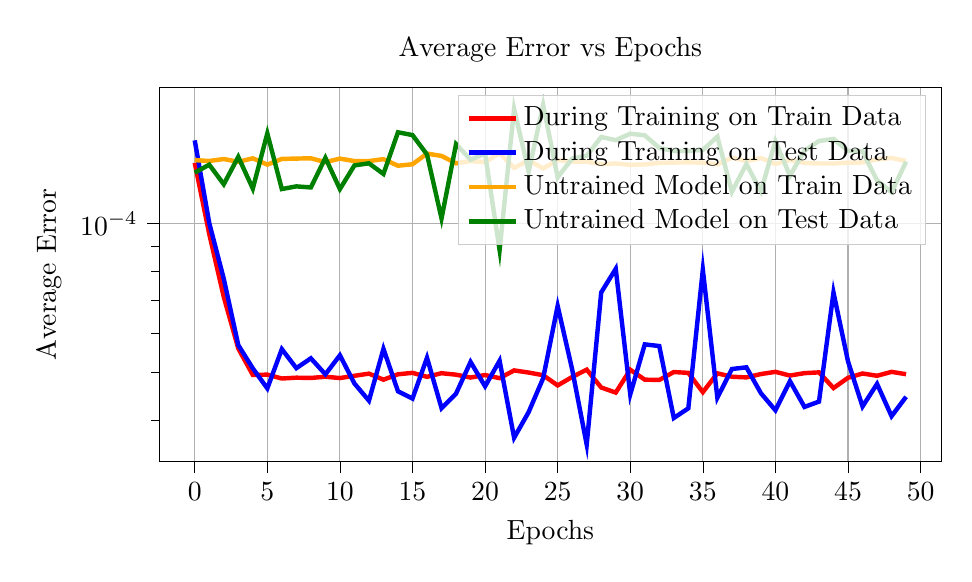
\begin{tikzpicture}

  \definecolor{darkgray176}{RGB}{176,176,176}
  \definecolor{green}{RGB}{0,128,0}
  \definecolor{lightgray204}{RGB}{204,204,204}
  \definecolor{orange}{RGB}{255,165,0}
  
  \begin{axis}[
    width = 0.95\textwidth,
    height = 18em,
  legend cell align={left},
  legend style={
    fill opacity=0.8,
    draw opacity=1,
    text opacity=1,
    % at={(0.91,0.5)},
    % anchor=east,
    draw=lightgray204
  },
  % log basis y={10},
  tick align=outside,
  tick pos=left,
  title={Average Error vs Epochs},
  x grid style={darkgray176},
  xlabel={Epochs},
  xmajorgrids,
  xmin=-2.45, xmax=51.45,
  xtick style={color=black},
  y grid style={darkgray176},
  ylabel={Average Error},
  ymajorgrids,
  ymin=3.30722135247185e-05, ymax=0.000188104234714924,
  ymode=log,
  ytick style={color=black},
  ytick={1e-06,1e-05,0.0001,0.001,0.01},
  yticklabels={
    \(\displaystyle {10^{-6}}\),
    \(\displaystyle {10^{-5}}\),
    \(\displaystyle {10^{-4}}\),
    \(\displaystyle {10^{-3}}\),
    \(\displaystyle {10^{-2}}\)
  }
  ]
  \addplot [ultra thick, red]
  table {%
  0 0.000132722096168436
  1 9.52958143898286e-05
  2 7.11312095518224e-05
  3 5.59525251446757e-05
  4 4.94734194944613e-05
  5 4.95356325700413e-05
  6 4.86540520796552e-05
  7 4.88426849187817e-05
  8 4.87789220642298e-05
  9 4.90620986965951e-05
  10 4.87564029754139e-05
  11 4.92705366923474e-05
  12 4.97732726216782e-05
  13 4.83878284285311e-05
  14 4.96224929520395e-05
  15 4.99510824738536e-05
  16 4.90340717078652e-05
  17 4.98722329211887e-05
  18 4.95317617605906e-05
  19 4.88754849357065e-05
  20 4.94462146889418e-05
  21 4.87317229271866e-05
  22 5.05235257151071e-05
  23 5.0024245865643e-05
  24 4.94094638270326e-05
  25 4.71192179247737e-05
  26 4.90080456074793e-05
  27 5.07079239469022e-05
  28 4.66571473225486e-05
  29 4.55734552815557e-05
  30 5.06827636854723e-05
  31 4.83968869957607e-05
  32 4.83256881125271e-05
  33 5.0144979468314e-05
  34 4.99464476888534e-05
  35 4.56594752904493e-05
  36 4.98443841934204e-05
  37 4.90569836983923e-05
  38 4.89077756355982e-05
  39 4.96737193316221e-05
  40 5.01869035360869e-05
  41 4.93312109028921e-05
  42 4.98860681545921e-05
  43 5.00653732160572e-05
  44 4.65431585325859e-05
  45 4.88188707095105e-05
  46 4.98049921588972e-05
  47 4.92811013828032e-05
  48 5.01822796650231e-05
  49 4.96389002364594e-05
  };
  \addlegendentry{During Training on Train Data}
  \addplot [ultra thick, blue]
  table {%
  0 0.000147356346133165
  1 0.000100276833109092
  2 7.74033032939769e-05
  3 5.68429713894147e-05
  4 5.10137870151084e-05
  5 4.64688382635359e-05
  6 5.57806524739135e-05
  7 5.1057828386547e-05
  8 5.34521313966252e-05
  9 4.96142783958931e-05
  10 5.42103043699171e-05
  11 4.7545585402986e-05
  12 4.38857059634756e-05
  13 5.58492865820881e-05
  14 4.58449612779077e-05
  15 4.43196513515431e-05
  16 5.35876279172953e-05
  17 4.23945093643852e-05
  18 4.53545399068389e-05
  19 5.25535251654219e-05
  20 4.69236656499561e-05
  21 5.28460477653425e-05
  22 3.69406589015853e-05
  23 4.16071488871239e-05
  24 4.87198121845722e-05
  25 6.8199158704374e-05
  26 5.0729689974105e-05
  27 3.57913850166369e-05
  28 7.26350262993947e-05
  29 8.1043537647929e-05
  30 4.51905725640245e-05
  31 5.70314368815161e-05
  32 5.65893242310267e-05
  33 4.04946149501484e-05
  34 4.23562341893557e-05
  35 8.07066462584771e-05
  36 4.44882716692518e-05
  37 5.08558587171137e-05
  38 5.12504157086369e-05
  39 4.54418550361879e-05
  40 4.19671923737042e-05
  41 4.80627386423294e-05
  42 4.26279038947541e-05
  43 4.37011694884859e-05
  44 7.25988211343065e-05
  45 5.26790354342666e-05
  46 4.27131417382043e-05
  47 4.74478620162699e-05
  48 4.08320811402518e-05
  49 4.46896556240972e-05
  };
  \addlegendentry{During Training on Test Data}
  \addplot [ultra thick, orange]
  table {%
  0 0.000134415182401426
  1 0.000133859735797159
  2 0.000135096372105181
  3 0.000133315537823364
  4 0.000135558802867308
  5 0.000131604872876778
  6 0.000135166221298277
  7 0.000135371694341302
  8 0.00013555760961026
  9 0.000133147303131409
  10 0.000135355425300077
  11 0.000133816851302981
  12 0.00013382603356149
  13 0.000135015754494816
  14 0.000130949250888079
  15 0.000131850087200291
  16 0.000138567527756095
  17 0.000137042501592077
  18 0.000132412038510665
  19 0.000133806184749119
  20 0.00013315056276042
  21 0.000138728239107877
  22 0.000129598542116582
  23 0.000134296817122959
  24 0.000129316467791796
  25 0.000134426998556592
  26 0.000133511028252542
  27 0.000133338689920492
  28 0.000131890992633998
  29 0.000132342014694586
  30 0.000131475171656348
  31 0.000131742417579517
  32 0.000132709450554103
  33 0.000132882501929998
  34 0.000132975561427884
  35 0.0001328465732513
  36 0.000131782973767258
  37 0.000135892565594986
  38 0.000133842084323987
  39 0.000135688576847315
  40 0.000132072207634337
  41 0.000134420246467926
  42 0.000132650457089767
  43 0.000132311062770896
  44 0.000132282293634489
  45 0.000132839733851142
  46 0.00013292086077854
  47 0.00013482163194567
  48 0.000135752008645795
  49 0.000133861845824867
  };
  \addlegendentry{Untrained Model on Train Data}
  \addplot [ultra thick, green]
  table {%
  0 0.00012677519407589
  1 0.000131578868604265
  2 0.000120126052934211
  3 0.000136456466862001
  4 0.000117726136522833
  5 0.000152216060087085
  6 0.000117487055831589
  7 0.000118944961286616
  8 0.000118362011562567
  9 0.000135828202473931
  10 0.000117471114208456
  11 0.000131132823298685
  12 0.0001324288896285
  13 0.00012603857612703
  14 0.000153000306454487
  15 0.000151011321577244
  16 0.000137982569867745
  17 0.000102457801403943
  18 0.000144789562909864
  19 0.0001346626522718
  20 0.00013855162251275
  21 8.84784312802367e-05
  22 0.000170658269780688
  23 0.000127359642647207
  24 0.000173813430592418
  25 0.000124067300930619
  26 0.000135398469865322
  27 0.000137087437906303
  28 0.00014967487368267
  29 0.000147490325616673
  30 0.000151992935570888
  31 0.000150832158396952
  32 0.000142279764986597
  33 0.000140183008625172
  34 0.000140295756864361
  35 0.000140935080708005
  36 0.000149868414155208
  37 0.000115996052045375
  38 0.000131940701976418
  39 0.000116244016680866
  40 0.000146826612763107
  41 0.000124963815324008
  42 0.000140456089866348
  43 0.000146886712173
  44 0.000148353181430139
  45 0.000140342046506703
  46 0.000139979019877501
  47 0.000122307494166307
  48 0.000115747614472639
  49 0.000133389243273996
  };
  \addlegendentry{Untrained Model on Test Data}
  \end{axis}
  
  \end{tikzpicture}
  
%   % \end{turn}
%   \caption{URWF scenario $0$, layers$=10$, epochs$=50$, learning rate$=10^{-3}$}
%     % \label{fig:wf_dfghvariants}
%   \end{figure}
% %   \clearpage % End the page
% }


% \afterpage{%
% %   \clearpage % Start a new page
%   \begin{figure}[!htbp]
%     \centering
% 	\captionsetup{justification=centering}
%   % \begin{turn}{-90}
%     % This file was created with tikzplotlib v0.10.1.
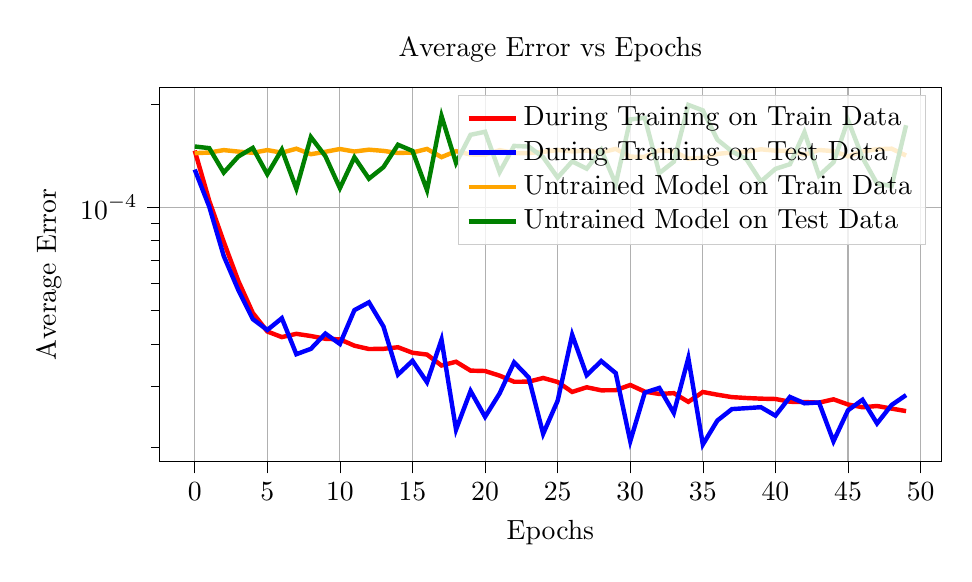
\begin{tikzpicture}

    \definecolor{darkgray176}{RGB}{176,176,176}
    \definecolor{green}{RGB}{0,128,0}
    \definecolor{lightgray204}{RGB}{204,204,204}
    \definecolor{orange}{RGB}{255,165,0}
    
    \begin{axis}[
      width = 0.95\textwidth,
      height = 18em,
    legend cell align={left},
    legend style={
      fill opacity=0.8,
      draw opacity=1,
      text opacity=1,
      % at={(0.91,0.5)},
      % anchor=east,
      draw=lightgray204
    },
    % log basis y={10},
    tick align=outside,
    tick pos=left,
    title={Average Error vs Epochs},
    x grid style={darkgray176},
    xlabel={Epochs},
    xmajorgrids,
    xmin=-2.45, xmax=51.45,
    xtick style={color=black},
    y grid style={darkgray176},
    ylabel={Average Error},
    ymajorgrids,
    ymin=1.81602095355054e-05, ymax=0.000222783350611656,
    ymode=log,
    ytick style={color=black},
    ytick={1e-06,1e-05,0.0001,0.001,0.01},
    yticklabels={
      \(\displaystyle {10^{-6}}\),
      \(\displaystyle {10^{-5}}\),
      \(\displaystyle {10^{-4}}\),
      \(\displaystyle {10^{-3}}\),
      \(\displaystyle {10^{-2}}\)
    }
    ]
    \addplot [ultra thick, red]
    table {%
    0 0.000146278194733895
    1 0.000104420905699953
    2 7.92681239545345e-05
    3 6.10758288530633e-05
    4 4.92224680783693e-05
    5 4.34550092904828e-05
    6 4.18473209720105e-05
    7 4.27740997110959e-05
    8 4.21492586610839e-05
    9 4.13740053772926e-05
    10 4.12062763643917e-05
    11 3.95096503780223e-05
    12 3.86323808925226e-05
    13 3.8685386243742e-05
    14 3.90951099689119e-05
    15 3.7674093618989e-05
    16 3.72231625078712e-05
    17 3.45841617672704e-05
    18 3.54710755345877e-05
    19 3.34202304657083e-05
    20 3.33290299749933e-05
    21 3.23112872138154e-05
    22 3.10100913338829e-05
    23 3.1028324883664e-05
    24 3.18035745294765e-05
    25 3.09636925521772e-05
    26 2.89666477328865e-05
    27 2.98817540169694e-05
    28 2.92815784632694e-05
    29 2.92987824650481e-05
    30 3.03483375319047e-05
    31 2.90223379124654e-05
    32 2.85742298729019e-05
    33 2.87294860754628e-05
    34 2.71037642960437e-05
    35 2.89524341496872e-05
    36 2.84268226096174e-05
    37 2.79751275229501e-05
    38 2.78087027254514e-05
    39 2.76841983577469e-05
    40 2.76240880339174e-05
    41 2.71164917649003e-05
    42 2.70670807367424e-05
    43 2.69537595158909e-05
    44 2.75629245152231e-05
    45 2.6622759833117e-05
    46 2.61352506640833e-05
    47 2.63559304585215e-05
    48 2.59002445091028e-05
    49 2.54677142947912e-05
    };
    \addlegendentry{During Training on Train Data}
    \addplot [ultra thick, blue]
    table {%
    0 0.000128779443912208
    1 0.00010038409527624
    2 7.20859316061251e-05
    3 5.74429686821532e-05
    4 4.72210740554146e-05
    5 4.38880924775731e-05
    6 4.74986336485017e-05
    7 3.7310368497856e-05
    8 3.86739084206056e-05
    9 4.2848852899624e-05
    10 3.9968599594431e-05
    11 5.0143735279562e-05
    12 5.285011138767e-05
    13 4.49300969194155e-05
    14 3.25484543282073e-05
    15 3.56887139787432e-05
    16 3.09173701680265e-05
    17 4.11355395044666e-05
    18 2.24964205699507e-05
    19 2.91467531496892e-05
    20 2.45067039941205e-05
    21 2.86695176328067e-05
    22 3.53258474206086e-05
    23 3.19383507303428e-05
    24 2.18671866605291e-05
    25 2.73038804152748e-05
    26 4.2485826270422e-05
    27 3.24111788359005e-05
    28 3.56320124410558e-05
    29 3.28617716149893e-05
    30 2.08107903745258e-05
    31 2.8820493753301e-05
    32 2.97523602057481e-05
    33 2.5161634766846e-05
    34 3.63602011930197e-05
    35 2.03521376533899e-05
    36 2.3903059627628e-05
    37 2.58119016507408e-05
    38 2.59747375821462e-05
    39 2.61434706771979e-05
    40 2.47025800490519e-05
    41 2.80039475910598e-05
    42 2.68369312834693e-05
    43 2.69887150352588e-05
    44 2.07989851332968e-05
    45 2.56072144111386e-05
    46 2.74763297056779e-05
    47 2.34442468354246e-05
    48 2.65273101831554e-05
    49 2.83582612610189e-05
    };
    \addlegendentry{During Training on Test Data}
    \addplot [ultra thick, orange]
    table {%
    0 0.000143817727803253
    1 0.000144362973514944
    2 0.000146766687976196
    3 0.000145289624924771
    4 0.000144115459988825
    5 0.000146782738738693
    6 0.000144232981256209
    7 0.000148136517964303
    8 0.000142785676871426
    9 0.000145113124744967
    10 0.000147847051266581
    11 0.000145348269143142
    12 0.000147180369822308
    13 0.000145986239658669
    14 0.000143930912599899
    15 0.000144404504681006
    16 0.000147901533637196
    17 0.000139990574098192
    18 0.000145746729685925
    19 0.000142500211950392
    20 0.000142163597047329
    21 0.000146696082083508
    22 0.00014386406110134
    23 0.000143894605571404
    24 0.000145068916026503
    25 0.000146825681440532
    26 0.000145544589031488
    27 0.000146261707413942
    28 0.000144508856465109
    29 0.000147926708450541
    30 0.000140387055580504
    31 0.000140381875098683
    32 0.00014663758338429
    33 0.00014546888996847
    34 0.000138474060804583
    35 0.000139353855047375
    36 0.000143018041853793
    37 0.000144513905979693
    38 0.000145408208481967
    39 0.00014754910080228
    40 0.000146216785651632
    41 0.000146020873216912
    42 0.000142244753078558
    43 0.000146861115354113
    44 0.000145769605296664
    45 0.000140737523906864
    46 0.000145486628753133
    47 0.000147612619912252
    48 0.000148156919749454
    49 0.000141483877087012
    };
    \addlegendentry{Untrained Model on Train Data}
    \addplot [ultra thick, green]
    table {%
    0 0.000150364750879817
    1 0.000148715800605714
    2 0.000126212136819959
    3 0.000140571341034956
    4 0.00014891754835844
    5 0.0001248148328159
    6 0.000147257611388341
    7 0.000113281806989107
    8 0.000160188879817724
    9 0.000140890551847406
    10 0.000113709320430644
    11 0.000139861251227558
    12 0.00012114318087697
    13 0.000130904605612159
    14 0.000152134743984789
    15 0.000145973521284759
    16 0.000112183719465975
    17 0.000184424745384604
    18 0.000134632413391955
    19 0.00016261384007521
    20 0.000165981182362884
    21 0.00012655348109547
    22 0.000150970416143537
    23 0.000150248713907786
    24 0.000139949814183637
    25 0.000122067860502284
    26 0.000136034286697395
    27 0.000129538966575637
    28 0.000146950769703835
    29 0.000116940143925603
    30 0.000180271337740123
    31 0.000182227056939155
    32 0.000125736318295822
    33 0.000135748166940175
    34 0.000198789552086964
    35 0.000191611266927794
    36 0.000157448623212986
    37 0.000145551850437187
    38 0.000138119357870892
    39 0.000118853095045779
    40 0.000129383552120999
    41 0.000133493827888742
    42 0.00016541252261959
    43 0.000123607329442166
    44 0.000135195485199802
    45 0.000179384034709074
    46 0.000139412193675525
    47 0.00011720007751137
    48 0.000115313268906903
    49 0.000173394801095128
    };
    \addlegendentry{Untrained Model on Test Data}
    \end{axis}
    
    \end{tikzpicture}
    
%   % \end{turn}
%   \caption{URWF scenario $1$, layers$=10$, epochs$=50$, learning rate$=10^{-3}$}
%     % \label{fig:wf_dfghvariants}
%   \end{figure}
% %   \clearpage % End the page
% }


% \afterpage{%
% %   \clearpage % Start a new page
%   \begin{figure}[!htbp]
%     \centering
% 	\captionsetup{justification=centering}
%   % \begin{turn}{-90}
%     % This file was created with tikzplotlib v0.10.1.
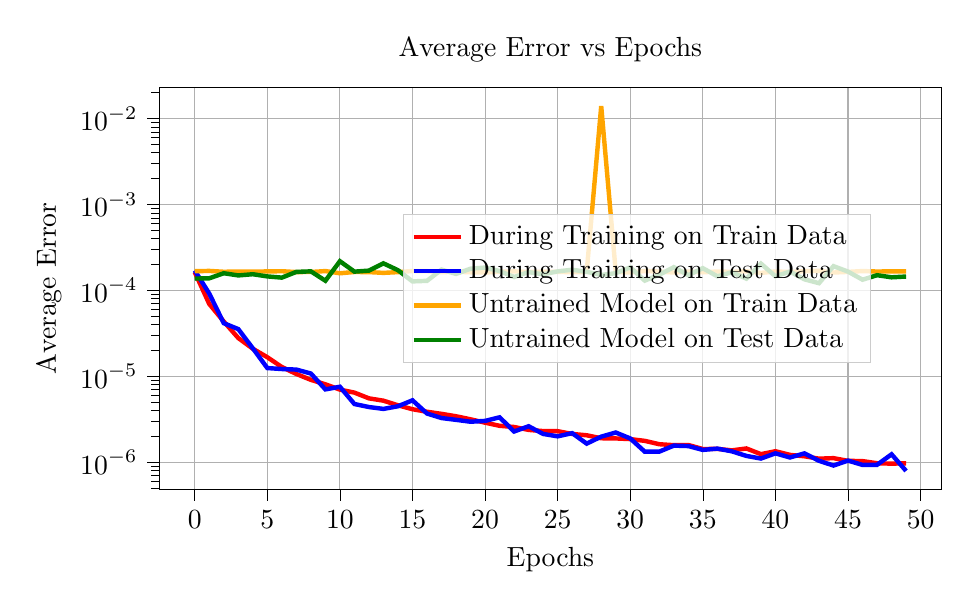
\begin{tikzpicture}

  \definecolor{darkgray176}{RGB}{176,176,176}
  \definecolor{green}{RGB}{0,128,0}
  \definecolor{lightgray204}{RGB}{204,204,204}
  \definecolor{orange}{RGB}{255,165,0}
  
  \begin{axis}[
    width = 0.95\textwidth,
    height = 19em,
  legend cell align={left},
  legend style={
    fill opacity=0.8,
    draw opacity=1,
    text opacity=1,
    at={(0.91,0.5)},
    anchor=east,
    draw=lightgray204
  },
  % log basis y={10},
  tick align=outside,
  tick pos=left,
  title={Average Error vs Epochs},
  x grid style={darkgray176},
  xlabel={Epochs},
  xmajorgrids,
  xmin=-2.45, xmax=51.45,
  xtick style={color=black},
  y grid style={darkgray176},
  ylabel={Average Error},
  ymajorgrids,
  ymin=4.86653883990184e-07, ymax=0.0227388191398161,
  ymode=log,
  ytick style={color=black},
  ytick={1e-08,1e-07,1e-06,1e-05,0.0001,0.001,0.01,0.1,1},
yticklabels={
  \(\displaystyle {10^{-8}}\),
  \(\displaystyle {10^{-7}}\),
  \(\displaystyle {10^{-6}}\),
  \(\displaystyle {10^{-5}}\),
  \(\displaystyle {10^{-4}}\),
  \(\displaystyle {10^{-3}}\),
  \(\displaystyle {10^{-2}}\),
  \(\displaystyle {10^{-1}}\),
  \(\displaystyle {10^{0}}\)
}
  ]
  \addplot [ultra thick, red]
table {%
0 0.000163097938639112
1 6.95640046615154e-05
2 4.34557296102867e-05
3 2.79197738564108e-05
4 2.09615609492175e-05
5 1.66988993441919e-05
6 1.28378760564374e-05
7 1.0652799574018e-05
8 9.10444123292109e-06
9 8.07891319709597e-06
10 7.00679311194108e-06
11 6.46568105366896e-06
12 5.54613734493614e-06
13 5.20814501214772e-06
14 4.60338424090878e-06
15 4.14187388741993e-06
16 3.87155705539044e-06
17 3.66023209608102e-06
18 3.43169858751935e-06
19 3.16300565827987e-06
20 2.88951900984102e-06
21 2.65776702690346e-06
22 2.57361512012722e-06
23 2.38001484831329e-06
24 2.30703153647482e-06
25 2.29981696975301e-06
26 2.13718476516078e-06
27 2.06161598725885e-06
28 1.90302205282933e-06
29 1.89487604984606e-06
30 1.86091483556083e-06
31 1.7752225858203e-06
32 1.62237029144308e-06
33 1.58172042574733e-06
34 1.58960199314606e-06
35 1.42605972541787e-06
36 1.43255817874888e-06
37 1.37571066716191e-06
38 1.44837963489408e-06
39 1.24299731396604e-06
40 1.34513811644865e-06
41 1.21901894090115e-06
42 1.17452839276666e-06
43 1.10200176095532e-06
44 1.11689780624147e-06
45 1.03926151950873e-06
46 1.03192769529414e-06
47 9.74933186626004e-07
48 9.63614297688764e-07
49 9.73476744547952e-07
};
\addlegendentry{During Training on Train Data}
\addplot [ultra thick, blue]
table {%
0 0.000170692641404457
1 9.19459635042585e-05
2 4.15414688177407e-05
3 3.54702751792502e-05
4 2.12094691960374e-05
5 1.24855350804864e-05
6 1.21629809655133e-05
7 1.19845199151314e-05
8 1.07882378870272e-05
9 7.0505338953808e-06
10 7.56783765609725e-06
11 4.76404329674551e-06
12 4.39399946117192e-06
13 4.18000399804441e-06
14 4.48639048045152e-06
15 5.26103758602403e-06
16 3.69247027265374e-06
17 3.27280577039346e-06
18 3.11769122163241e-06
19 2.96365715257707e-06
20 3.03114143207495e-06
21 3.33551702169643e-06
22 2.28128169510455e-06
23 2.62626690528123e-06
24 2.1363327959989e-06
25 2.00401018446428e-06
26 2.18199670598551e-06
27 1.64860466611572e-06
28 1.9884250832547e-06
29 2.22067751565191e-06
30 1.89409990980494e-06
31 1.32749971726298e-06
32 1.33019966597203e-06
33 1.56249666360964e-06
34 1.54365932303335e-06
35 1.39256223974371e-06
36 1.44203693253075e-06
37 1.34115566652326e-06
38 1.18524599201919e-06
39 1.10521705209976e-06
40 1.27091846024996e-06
41 1.1371939763194e-06
42 1.26946542877704e-06
43 1.04059097338904e-06
44 9.16003955353517e-07
45 1.04647676835157e-06
46 9.31057911657263e-07
47 9.34875686198211e-07
48 1.23812992569583e-06
49 7.93363767570554e-07
};
\addlegendentry{During Training on Test Data}
\addplot [ultra thick, orange]
table {%
0 0.000167268663062714
1 0.000168611761182547
2 0.000164750032126904
3 0.000166074707522057
4 0.000165510311489925
5 0.000166329540661536
6 0.000167264486663043
7 0.000163467208039947
8 0.000163789329235442
9 0.000167902631801553
10 0.000158251743414439
11 0.000163772841915488
12 0.000163379823789001
13 0.000159947972861119
14 0.000163212345796637
15 0.000168250291608274
16 0.000167275851708837
17 0.00016272951324936
18 0.000165133300470188
19 0.000162475116667338
20 0.000161717063747346
21 0.000164484881679527
22 0.000166474826983176
23 0.000163901393534616
24 0.00016524524835404
25 0.000164450189913623
26 0.000162684242241085
27 0.000163810182129964
28 0.0139481220394373
29 0.00016462522034999
30 0.000161635733093135
31 0.000168101963936351
32 0.000165689591085538
33 0.000161484422278591
34 0.000165562189067714
35 0.000162491676746868
36 0.000165928257047199
37 0.000164456811035052
38 0.000166921367053874
39 0.000159998307935894
40 0.000166102094226517
41 0.000163806194905192
42 0.000167545396834612
43 0.000168941318406723
44 0.000161504111019894
45 0.000164178913109936
46 0.000167981517734006
47 0.000165818899404258
48 0.000166785175679252
49 0.000166209385497496
};
\addlegendentry{Untrained Model on Train Data}
\addplot [ultra thick, green]
table {%
0 0.000137429335154593
1 0.000138295567012392
2 0.000158476585056633
3 0.000149381274241023
4 0.000154329158249311
5 0.000145530575537123
6 0.000140856049256399
7 0.000164252924150787
8 0.000166630212333985
9 0.000129618609207682
10 0.000218662316910923
11 0.000165390243637376
12 0.000169930906849913
13 0.000206377269933
14 0.00017179134010803
15 0.000127295410493389
16 0.000129273044876754
17 0.000174764529219829
18 0.000155563189764507
19 0.00017893330368679
20 0.00018444396846462
21 0.000167917532962747
22 0.000143270124681294
23 0.000163351345690899
24 0.000153900356963277
25 0.000166609228472225
26 0.000174030355992727
27 0.000164638928254135
28 0.000151140950038098
29 0.000158716487931088
30 0.000185446187970228
31 0.000130001790239476
32 0.000152179549331777
33 0.000186295816092752
34 0.000150395178934559
35 0.000181550378329121
36 0.000145733851240948
37 0.000162864715093747
38 0.00013712968211621
39 0.000205252305022441
40 0.000145977654028684
41 0.000165515957633033
42 0.000134605827042833
43 0.000121332785056438
44 0.00019154827168677
45 0.000165487450431101
46 0.00013320310972631
47 0.000150331645272672
48 0.000142030883580446
49 0.000145056197652593
};
\addlegendentry{Untrained Model on Test Data}
\end{axis}

\end{tikzpicture}
%   % \end{turn}
%   \caption{URWF scenario $2$, layers$=10$, epochs$=50$, learning rate$=10^{-3}$}
%     % \label{fig:wf_dfghvariants}
%   \end{figure}
% %   \clearpage % End the page
% }
% \afterpage{%
% %   \clearpage % Start a new page
%   \begin{figure}[!htbp]
%     \centering
% 	\captionsetup{justification=centering}
%   % \begin{turn}{-90}
%     % This file was created with tikzplotlib v0.10.1.
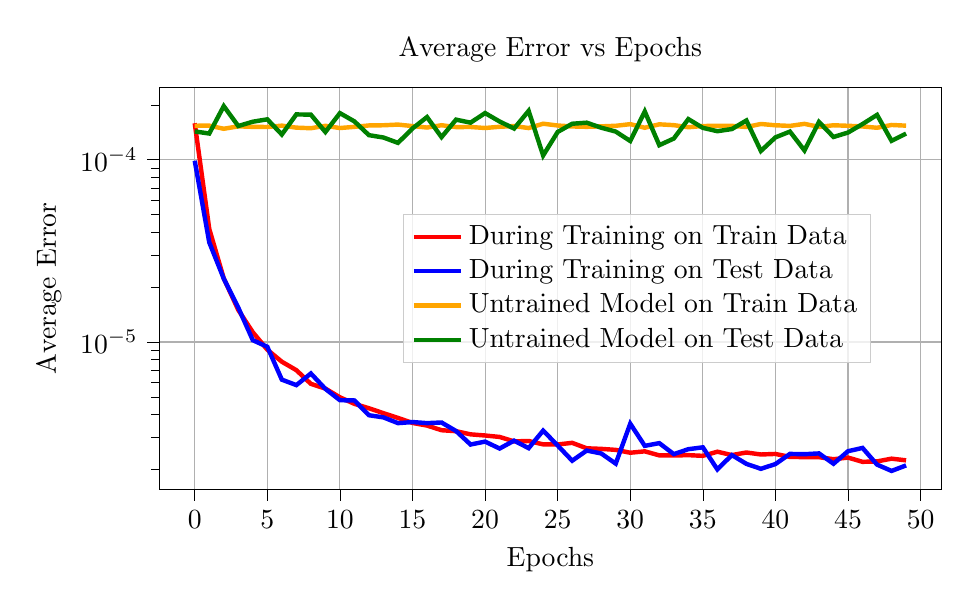
\begin{tikzpicture}

  \definecolor{darkgray176}{RGB}{176,176,176}
  \definecolor{green}{RGB}{0,128,0}
  \definecolor{lightgray204}{RGB}{204,204,204}
  \definecolor{orange}{RGB}{255,165,0}
  
  \begin{axis}[
    width = 0.95\textwidth,
    height = 19em,
  legend cell align={left},
  legend style={
    fill opacity=0.8,
    draw opacity=1,
    text opacity=1,
    at={(0.91,0.5)},
    anchor=east,
    draw=lightgray204
  },
  % log basis y={10},
  tick align=outside,
  tick pos=left,
  title={Average Error vs Epochs},
  x grid style={darkgray176},
  xlabel={Epochs},
  xmajorgrids,
  xmin=-2.45, xmax=51.45,
  xtick style={color=black},
  y grid style={darkgray176},
  ylabel={Average Error},
  ymajorgrids,
  ymin=1.55984612605889e-06, ymax=0.000247681245738091,
ymode=log,
ytick style={color=black},
ytick={1e-07,1e-06,1e-05,0.0001,0.001,0.01},
yticklabels={
  \(\displaystyle {10^{-7}}\),
  \(\displaystyle {10^{-6}}\),
  \(\displaystyle {10^{-5}}\),
  \(\displaystyle {10^{-4}}\),
  \(\displaystyle {10^{-3}}\),
  \(\displaystyle {10^{-2}}\)
}
  ]
  \addplot [ultra thick, red]
table {%
0 0.000158629423822276
1 4.17500705225393e-05
2 2.23410734179197e-05
3 1.49923098433646e-05
4 1.13186724775005e-05
5 9.07615412870655e-06
6 7.79907350079156e-06
7 7.01064618624514e-06
8 5.89603132539196e-06
9 5.5544014685438e-06
10 4.97701785207028e-06
11 4.58103113487596e-06
12 4.33344484918052e-06
13 4.07163042837055e-06
14 3.83643191526062e-06
15 3.59927594217879e-06
16 3.48308049069601e-06
17 3.28366763824306e-06
18 3.24376105709234e-06
19 3.11671965391724e-06
20 3.07204231830838e-06
21 3.01650766232342e-06
22 2.8517763439595e-06
23 2.86554063677613e-06
24 2.74647231890413e-06
25 2.74263447863632e-06
26 2.79981736639456e-06
27 2.61375680565834e-06
28 2.59432090388145e-06
29 2.56180942415085e-06
30 2.47075331571978e-06
31 2.5146134703391e-06
32 2.38996767620847e-06
33 2.38629627347109e-06
34 2.39670816881699e-06
35 2.37572703554179e-06
36 2.50309471994115e-06
37 2.3985255666048e-06
38 2.47841694545059e-06
39 2.41662883126992e-06
40 2.43350336859294e-06
41 2.34371736951289e-06
42 2.33795276471938e-06
43 2.33626451517921e-06
44 2.27647865358449e-06
45 2.32412526202097e-06
46 2.20256538341346e-06
47 2.21448135562241e-06
48 2.2928848011361e-06
49 2.24423251893313e-06
};
\addlegendentry{During Training on Train Data}
\addplot [ultra thick, blue]
table {%
0 9.87597886705771e-05
1 3.5224966268288e-05
2 2.22798680624692e-05
3 1.54417248268146e-05
4 1.02357944342657e-05
5 9.41831694944995e-06
6 6.21941171630169e-06
7 5.80472351430217e-06
8 6.72237501930795e-06
9 5.53433847017004e-06
10 4.79677191833616e-06
11 4.78111951451865e-06
12 3.96789118894958e-06
13 3.8617140489805e-06
14 3.59103978553321e-06
15 3.64064408131526e-06
16 3.59160890184285e-06
17 3.62066725756449e-06
18 3.25107043863682e-06
19 2.74062654170848e-06
20 2.84425550489686e-06
21 2.60542879004788e-06
22 2.87777834273584e-06
23 2.617919108161e-06
24 3.26798544847406e-06
25 2.70756140707817e-06
26 2.23450524572399e-06
27 2.53932171290217e-06
28 2.44782427216705e-06
29 2.15366708289366e-06
30 3.5666532767209e-06
31 2.6958002763422e-06
32 2.78928996522154e-06
33 2.4274806946778e-06
34 2.58378622675082e-06
35 2.64566619989637e-06
36 2.00250156012771e-06
37 2.39911287280847e-06
38 2.14669603337825e-06
39 2.01651187126117e-06
40 2.1419243694254e-06
41 2.43437216340681e-06
42 2.42601004174503e-06
43 2.44980583374854e-06
44 2.15043269236048e-06
45 2.5189995085384e-06
46 2.62520006799605e-06
47 2.1261782876536e-06
48 1.96389669326891e-06
49 2.10574557968357e-06
};
\addlegendentry{During Training on Test Data}
\addplot [ultra thick, orange]
table {%
0 0.000153553526615724
1 0.0001537842763355
2 0.000147777231177315
3 0.00015241838991642
4 0.00015136860019993
5 0.00015115799033083
6 0.000153794055222534
7 0.000149910119944252
8 0.000148827923112549
9 0.000153429486090317
10 0.000149183717439882
11 0.000151428583194502
12 0.000154140201630071
13 0.000154504115926102
14 0.000155849425937049
15 0.000152900945977308
16 0.000150118707097135
17 0.000154557346832007
18 0.000150987645611167
19 0.00015114396228455
20 0.000149241168401204
21 0.000151554413605481
22 0.00015294119657483
23 0.000149149796925485
24 0.00015752662147861
25 0.000154035544255748
26 0.000152168999193236
27 0.000151451749843545
28 0.000152411332237534
29 0.000153456567204557
30 0.000156663649249822
31 0.000149743806105107
32 0.000156316513312049
33 0.000154719615238719
34 0.000150691892486066
35 0.000153021101141348
36 0.000153451750520617
37 0.000153334884089418
38 0.000151146596181206
39 0.000157007118104957
40 0.000154453708091751
41 0.000153273300384171
42 0.000157264556037262
43 0.000151349857333116
44 0.000154477093019523
45 0.000153465225594118
46 0.000152173946844414
47 0.000149670915561728
48 0.000155075787915848
49 0.000153709916048683
};
\addlegendentry{Untrained Model on Train Data}
\addplot [ultra thick, green]
table {%
0 0.000142935779877007
1 0.000139173978823237
2 0.000196723500266671
3 0.00015302310930565
4 0.000161568226758391
5 0.000166518264450133
6 0.000137492650537752
7 0.000177166191861033
8 0.000176630361238495
9 0.000141880940645933
10 0.000180077680852264
11 0.000162175492732786
12 0.000136325703351758
13 0.000132341476273723
14 0.000123682111734524
15 0.000148397040902637
16 0.00017129372281488
17 0.00013302119623404
18 0.000165837176609784
19 0.000159636896569282
20 0.000180231349077076
21 0.000162036085384898
22 0.000148200779221952
23 0.000185301920282654
24 0.000105486673419364
25 0.000141921264003031
26 0.000157471571583301
27 0.000159628689289093
28 0.000149803585372865
29 0.000142626580782235
30 0.000126621496747248
31 0.000183925643796101
32 0.000120122444059234
33 0.000130652289954014
34 0.000166988946148194
35 0.000149514860822819
36 0.000143318276968785
37 0.000147275306517258
38 0.000164102355483919
39 0.000111702123831492
40 0.000132550703710876
41 0.000142650460475124
42 0.000112421752419323
43 0.000161090036272071
44 0.000133249923237599
45 0.000140913631184958
46 0.000156887806952
47 0.000176143701537512
48 0.000126888087834232
49 0.000139085881528445
};
\addlegendentry{Untrained Model on Test Data}
\end{axis}

\end{tikzpicture}

%   % \end{turn}
%   \caption{URWF scenario $3$, layers$=10$, epochs$=50$, learning rate$=10^{-3}$}
%     % \label{fig:wf_dfghvariants}
%   \end{figure}
% %   \clearpage % End the page
% }
% \afterpage{%
% %   \clearpage % Start a new page
%   \begin{figure}[!htbp]
%     \centering
% 	\captionsetup{justification=centering}
%   % \begin{turn}{-90}
%     % This file was created with tikzplotlib v0.10.1.
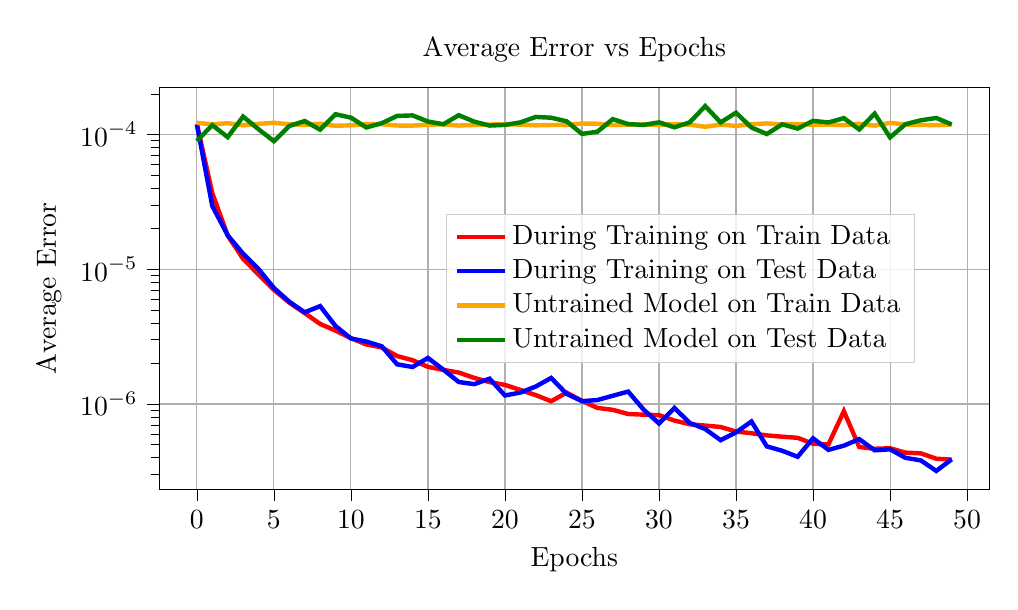
\begin{tikzpicture}

  \definecolor{darkgray176}{RGB}{176,176,176}
  \definecolor{green}{RGB}{0,128,0}
  \definecolor{lightgray204}{RGB}{204,204,204}
  \definecolor{orange}{RGB}{255,165,0}
  
  \begin{axis}[
    width = 1.0\textwidth,
    height = 19em,
  legend cell align={left},
  legend style={
    fill opacity=0.8,
    draw opacity=1,
    text opacity=1,
    at={(0.91,0.5)},
    anchor=east,
    draw=lightgray204
  },
  % log basis y={10},
  tick align=outside,
  tick pos=left,
  title={Average Error vs Epochs},
  x grid style={darkgray176},
  xlabel={Epochs},
  xmajorgrids,
  xmin=-2.45, xmax=51.45,
  xtick style={color=black},
  y grid style={darkgray176},
  ylabel={Average Error},
  ymajorgrids,
  ymin=2.33510655990556e-07, ymax=0.000221454230592227,
  ymode=log,
  ytick style={color=black},
  ytick={1e-08,1e-07,1e-06,1e-05,0.0001,0.001,0.01},
  yticklabels={
    \(\displaystyle {10^{-8}}\),
    \(\displaystyle {10^{-7}}\),
    \(\displaystyle {10^{-6}}\),
    \(\displaystyle {10^{-5}}\),
    \(\displaystyle {10^{-4}}\),
    \(\displaystyle {10^{-3}}\),
    \(\displaystyle {10^{-2}}\)
  }
  ]
  \addplot [ultra thick, red]
table {%
0 0.000119110678497236
1 3.66446620319039e-05
2 1.77629917743616e-05
3 1.19415099106845e-05
4 9.14171869226266e-06
5 7.0352730290324e-06
6 5.64817901249626e-06
7 4.72462261313922e-06
8 3.92743004340446e-06
9 3.50450204678054e-06
10 3.07970799440227e-06
11 2.76725950243417e-06
12 2.6275106392859e-06
13 2.26941324399377e-06
14 2.1133414520591e-06
15 1.88730939498782e-06
16 1.79045071035944e-06
17 1.71247768321336e-06
18 1.56285193497752e-06
19 1.45354010783194e-06
20 1.38544032779464e-06
21 1.27156704365916e-06
22 1.16367743885348e-06
23 1.04827813629527e-06
24 1.21447124001861e-06
25 1.05589560916997e-06
26 9.35082709929702e-07
27 9.04937735413114e-07
28 8.4294913449412e-07
29 8.33415299439366e-07
30 8.2679014212772e-07
31 7.54069617414643e-07
32 7.0767163151686e-07
33 6.91661682594713e-07
34 6.75471369504521e-07
35 6.25178131485882e-07
36 6.06936112035328e-07
37 5.85125235375017e-07
38 5.72119461139664e-07
39 5.61235140139615e-07
40 5.07119239046006e-07
41 5.00920407375816e-07
42 8.84193866568239e-07
43 4.79913239814778e-07
44 4.65450710862569e-07
45 4.69535621050454e-07
46 4.35870873616295e-07
47 4.30478280577518e-07
48 3.92834294871136e-07
49 3.87007872859613e-07
};
\addlegendentry{During Training on Train Data}
\addplot [ultra thick, blue]
table {%
0 0.00011835517216241
1 2.94239616778214e-05
2 1.78588288690662e-05
3 1.30369371618144e-05
4 1.00456127256621e-05
5 7.25863583284081e-06
6 5.73770012124442e-06
7 4.78903893963434e-06
8 5.3246581046551e-06
9 3.79064999833645e-06
10 3.06249035020301e-06
11 2.90575530925707e-06
12 2.68139638137654e-06
13 1.96956534637138e-06
14 1.88275339496613e-06
15 2.19661774281121e-06
16 1.79826713520015e-06
17 1.4568524875358e-06
18 1.40323015784816e-06
19 1.54136819219275e-06
20 1.15701266167889e-06
21 1.21596463031892e-06
22 1.34871140744508e-06
23 1.56057183176017e-06
24 1.1893879445779e-06
25 1.04965113223443e-06
26 1.07065557131136e-06
27 1.15161412850284e-06
28 1.23654535855167e-06
29 9.09538812265964e-07
30 7.17409648132161e-07
31 9.34473348479514e-07
32 7.23355014997651e-07
33 6.52248786536802e-07
34 5.39273003141716e-07
35 6.15782823842892e-07
36 7.42191218705557e-07
37 4.84830366076494e-07
38 4.49736944574397e-07
39 4.06152423693129e-07
40 5.56371048787696e-07
41 4.5693556671722e-07
42 4.90936429287103e-07
43 5.4913465419304e-07
44 4.53623528073877e-07
45 4.61155707398575e-07
46 3.98803734924513e-07
47 3.81665216764304e-07
48 3.18877482641255e-07
49 3.88750692081885e-07
};
\addlegendentry{During Training on Test Data}
\addplot [ultra thick, orange]
table {%
0 0.000121821271022782
1 0.000118786163511686
2 0.000121117249364033
3 0.000116916286060587
4 0.000119748343422543
5 0.000122004646982532
6 0.000118965377623681
7 0.000117821851745248
8 0.000119930613436736
9 0.000115926952275913
10 0.000116842471470591
11 0.000119264717795886
12 0.000119227319373749
13 0.000116418617835734
14 0.000116268653073348
15 0.000118152944196481
16 0.00011861881648656
17 0.000116357769002207
18 0.00011766472744057
19 0.000118461459351238
20 0.000118882810056675
21 0.000118203533929773
22 0.000116807641461492
23 0.000117445903015323
24 0.000117745250463486
25 0.000120490200060885
26 0.000120022261398844
27 0.000117423332994804
28 0.000118374497105833
29 0.000118564435979351
30 0.000118055919301696
31 0.000119002019346226
32 0.00011823955719592
33 0.000113942514872178
34 0.000118257907161023
35 0.00011569067282835
36 0.0001189872782561
37 0.000120693657663651
38 0.000118456307973247
39 0.000119453776278533
40 0.000117906849482097
41 0.000118281546747312
42 0.000117204755952116
43 0.000119701318908483
44 0.000116234936285764
45 0.000121639255667105
46 0.000118501353426836
47 0.000117697200039402
48 0.000117044612125028
49 0.000118546777230222
};
\addlegendentry{Untrained Model on Train Data}
\addplot [ultra thick, green]
table {%
0 8.94988697837107e-05
1 0.000117215560749173
2 9.54625502345152e-05
3 0.000135665308334865
4 0.000109265492937993
5 8.90656738192774e-05
6 0.00011553819058463
7 0.000125691731227562
8 0.000108503714727703
9 0.000141213327879086
10 0.000133093009935692
11 0.000112687819637358
12 0.000121152006613556
13 0.000137145310873166
14 0.000138392802909948
15 0.000124624843010679
16 0.000119010474008974
17 0.000138825504109263
18 0.000124459256767295
19 0.000116323259135243
20 0.000117673094791826
21 0.000122827914310619
22 0.000134805915877223
23 0.000133034307509661
24 0.000125141465105116
25 0.000100915800430812
26 0.000104666156403255
27 0.000129874431877397
28 0.000119255695608445
29 0.000117647301522084
30 0.000122925484902225
31 0.0001129619195126
32 0.000122985773487017
33 0.000162168624228798
34 0.000122765937703662
35 0.000144833509693854
36 0.000112565423478372
37 0.000100688113889191
38 0.000118868752906565
39 0.000110469525679946
40 0.00012610036355909
41 0.000122617464512587
42 0.000132143803057261
43 0.000108827247458976
44 0.000142696153488941
45 9.50354224187322e-05
46 0.000119124881166499
47 0.000127313265693374
48 0.000132477522129193
49 0.000118570867925882
};
\addlegendentry{Untrained Model on Test Data}
\end{axis}

\end{tikzpicture}
%   % \end{turn}
%   \caption{URWF scenario $4$, layers$=10$, epochs$=50$, learning rate$=10^{-3}$}
%     % \label{fig:wf_dfghvariants}
%   \end{figure}
% %   \clearpage % End the page
% }
% \afterpage{%
% %   \clearpage % Start a new page
%   \begin{figure}[!htbp]
%     \centering
% 	\captionsetup{justification=centering}
%   % \begin{turn}{-90}
%     % This file was created with tikzplotlib v0.10.1.
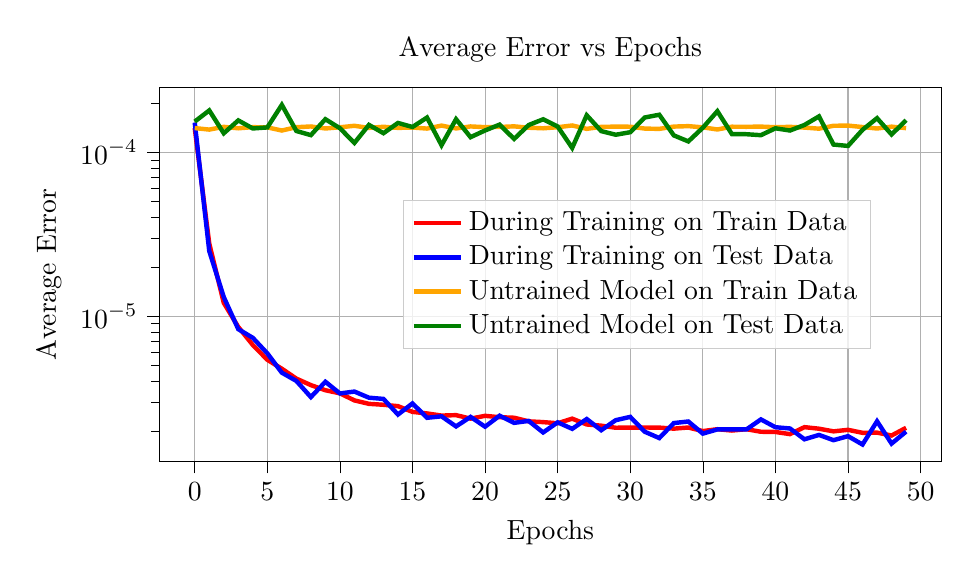
\begin{tikzpicture}

  \definecolor{darkgray176}{RGB}{176,176,176}
  \definecolor{green}{RGB}{0,128,0}
  \definecolor{lightgray204}{RGB}{204,204,204}
  \definecolor{orange}{RGB}{255,165,0}
  
  \begin{axis}[
    width = 0.95\textwidth,
    height = 18em,
  legend cell align={left},
  legend style={
    fill opacity=0.8,
    draw opacity=1,
    text opacity=1,
    at={(0.91,0.5)},
    anchor=east,
    draw=lightgray204
  },
  % log basis y={10},
  tick align=outside,
  tick pos=left,
  title={Average Error vs Epochs},
  x grid style={darkgray176},
  xlabel={Epochs},
  xmajorgrids,
  xmin=-2.45, xmax=51.45,
  xtick style={color=black},
  y grid style={darkgray176},
  ylabel={Average Error},
  ymajorgrids,
  ymin=1.30004957183654e-06, ymax=0.000247303366693065,
  ymode=log,
  ytick style={color=black},
  ytick={1e-07,1e-06,1e-05,0.0001,0.001,0.01},
  yticklabels={
  \(\displaystyle {10^{-7}}\),
  \(\displaystyle {10^{-6}}\),
  \(\displaystyle {10^{-5}}\),
  \(\displaystyle {10^{-4}}\),
  \(\displaystyle {10^{-3}}\),
  \(\displaystyle {10^{-2}}\)
}
  ]
  \addplot [ultra thick, red]
table {%
0 0.000140808770083822
1 2.77877024927875e-05
2 1.20650438475423e-05
3 8.60371164890239e-06
4 6.67991025693482e-06
5 5.42634415978682e-06
6 4.78406172987889e-06
7 4.16472585129668e-06
8 3.80176584258152e-06
9 3.53676637132594e-06
10 3.38710992764391e-06
11 3.06654351334146e-06
12 2.92217282549245e-06
13 2.88355204247637e-06
14 2.82838118437212e-06
15 2.60954288933135e-06
16 2.55327290688001e-06
17 2.47778302764345e-06
18 2.49293429988029e-06
19 2.37284029935836e-06
20 2.46894796873676e-06
21 2.42158648688928e-06
22 2.4035755359364e-06
23 2.28525459533557e-06
24 2.26031443162356e-06
25 2.22407220462628e-06
26 2.37349354392791e-06
27 2.18677610064333e-06
28 2.15019440474862e-06
29 2.08874439522333e-06
30 2.09293762054585e-06
31 2.09529321182345e-06
32 2.09285894925415e-06
33 2.06235563382506e-06
34 2.09541235562938e-06
35 1.99298551706306e-06
36 2.04654361368739e-06
37 2.00757085622172e-06
38 2.0461657186388e-06
39 1.97414806279994e-06
40 1.96775522454118e-06
41 1.90975492841972e-06
42 2.10623920793296e-06
43 2.06045660888776e-06
44 1.98512111637683e-06
45 2.02815704142267e-06
46 1.94528092833934e-06
47 1.95024335880589e-06
48 1.87281955277285e-06
49 2.08697565540206e-06
};
\addlegendentry{During Training on Train Data}
\addplot [ultra thick, blue]
table {%
0 0.000151866624946706
1 2.49946006078972e-05
2 1.30948674268438e-05
3 8.34122874948662e-06
4 7.38843755243579e-06
5 5.93867616771604e-06
6 4.52684344054433e-06
7 4.03162584916572e-06
8 3.21297193295322e-06
9 3.98407746615703e-06
10 3.38162840307632e-06
11 3.47228137798083e-06
12 3.18590946335462e-06
13 3.13101372739766e-06
14 2.51418100560841e-06
15 2.93958305519482e-06
16 2.4015394046728e-06
17 2.45178125624079e-06
18 2.12747499972465e-06
19 2.4323815068783e-06
20 2.11953897633066e-06
21 2.47359025706828e-06
22 2.23747611016734e-06
23 2.29793567996239e-06
24 1.95504912881006e-06
25 2.2525521217176e-06
26 2.05718492907181e-06
27 2.36007554121898e-06
28 2.01702164304152e-06
29 2.32281195167161e-06
30 2.43284330281313e-06
31 1.97447093341907e-06
32 1.80655024450971e-06
33 2.23063898374676e-06
34 2.27990972234693e-06
35 1.92346169569646e-06
36 2.03991839953233e-06
37 2.03988429348101e-06
38 2.03888680516684e-06
39 2.34781578001275e-06
40 2.10382722798386e-06
41 2.0672875962191e-06
42 1.77587082816899e-06
43 1.88824776614638e-06
44 1.75387231138302e-06
45 1.85520821105456e-06
46 1.65030076004768e-06
47 2.28701583182556e-06
48 1.67188488831016e-06
49 1.97793519873812e-06
};
\addlegendentry{During Training on Test Data}
\addplot [ultra thick, orange]
table {%
0 0.00014060313696973
1 0.000137656141305342
2 0.000143065073643811
3 0.000140192554681562
4 0.000142427845275961
5 0.000142034099553712
6 0.000135852737003006
7 0.00014235639537219
8 0.000143847602885216
9 0.00013983370445203
10 0.000142199758556671
11 0.000145203914144076
12 0.00014099404506851
13 0.000143194061820395
14 0.000140986638143659
15 0.000141734140925109
16 0.000139620620757341
17 0.000145604368299246
18 0.000139923329697922
19 0.000143899538670667
20 0.000142461081850342
21 0.000142865843372419
22 0.000144075427670032
23 0.000141339376568794
24 0.000140182426548563
25 0.000142293807584792
26 0.000145876678288914
27 0.000139112686156295
28 0.000143021941767074
29 0.000143526252941228
30 0.000143316239700653
31 0.000139636162202805
32 0.000139017691253684
33 0.000143602766911499
34 0.000144505393109284
35 0.000142094271723181
36 0.000137869006721303
37 0.000143355937325396
38 0.000143186174682342
39 0.000143536293762736
40 0.000142327175126411
41 0.000143050288897939
42 0.00014157967234496
43 0.000139441690407693
44 0.000145230937050655
45 0.000145648096804507
46 0.000142689401400276
47 0.000139756724820472
48 0.000143463927088305
49 0.00014049097080715
};
\addlegendentry{Untrained Model on Train Data}
\addplot [ultra thick, green]
table {%
0 0.000154029330587946
1 0.000180180853931233
2 0.000130726533825509
3 0.000156632129801437
4 0.000139883763040416
5 0.000141912765684538
6 0.000194816995644942
7 0.000135004651383497
8 0.000127355684526265
9 0.000159308925503865
10 0.000140322328661568
11 0.000114190057502128
12 0.000147035854752176
13 0.00013088078412693
14 0.000151125670527108
15 0.000142780350870453
16 0.000163049713592045
17 0.000110557492007501
18 0.00015931720554363
19 0.000123746853205375
20 0.00013601804676
21 0.000147675746120512
22 0.000120715449156705
23 0.000146728663821705
24 0.000159101778990589
25 0.000143717334140092
26 0.00010641503467923
27 0.000168388287420385
28 0.000134773305035196
29 0.000128033978398889
30 0.000132704633870162
31 0.00016315164975822
32 0.000169641323736869
33 0.000126891216496006
34 0.000116580682515632
35 0.000141325872391462
36 0.000178295289515518
37 0.000129308318719268
38 0.00012899779540021
39 0.000127264560433105
40 0.000140162432217039
41 0.000135849215439521
42 0.000146909078466706
43 0.000165729303262196
44 0.00011155797255924
45 0.000109411274024751
46 0.000137256662128493
47 0.00016158472863026
48 0.000128560437588021
49 0.000157007976667956
};
\addlegendentry{Untrained Model on Test Data}
\end{axis}

\end{tikzpicture}
%   % \end{turn}
%   \caption{URWF scenario $5$, layers$=10$, epochs$=50$, learning rate$=10^{-3}$}
%     % \label{fig:wf_dfghvariants}
%   \end{figure}
% %   \clearpage % End the page
% }
% \afterpage{%
% %   \clearpage % Start a new page
%   \begin{figure}[!htbp]
%     \centering
% 	\captionsetup{justification=centering}
%   % \begin{turn}{-90}
%     % This file was created with tikzplotlib v0.10.1.
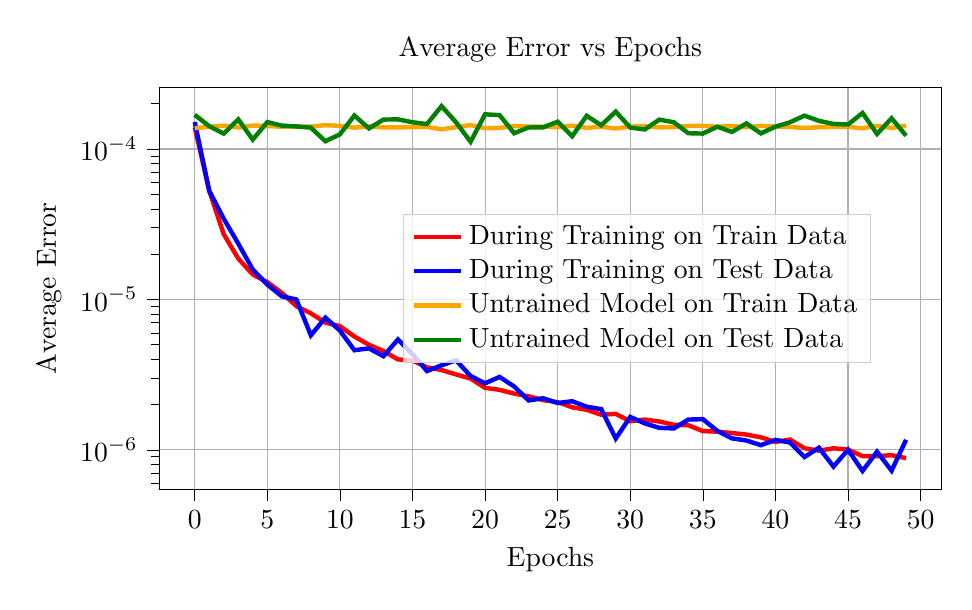
\begin{tikzpicture}

  \definecolor{darkgray176}{RGB}{176,176,176}
  \definecolor{green}{RGB}{0,128,0}
  \definecolor{lightgray204}{RGB}{204,204,204}
  \definecolor{orange}{RGB}{255,165,0}
  
  \begin{axis}[
    width = 0.95\textwidth,
    height = 19em,
  legend cell align={left},
  legend style={
    fill opacity=0.8,
    draw opacity=1,
    text opacity=1,
    at={(0.91,0.5)},
    anchor=east,
    draw=lightgray204
  },
  % log basis y={10},
  tick align=outside,
  tick pos=left,
  title={Average Error vs Epochs},
  x grid style={darkgray176},
  xlabel={Epochs},
  xmajorgrids,
  xmin=-2.45, xmax=51.45,
  xtick style={color=black},
  y grid style={darkgray176},
  ylabel={Average Error},
  ymajorgrids,
  ymin=5.47956319196448e-07, ymax=0.000254691381547786,
  ymode=log,
  ytick style={color=black},
  ytick={1e-08,1e-07,1e-06,1e-05,0.0001,0.001,0.01},
  yticklabels={
    \(\displaystyle {10^{-8}}\),
    \(\displaystyle {10^{-7}}\),
    \(\displaystyle {10^{-6}}\),
    \(\displaystyle {10^{-5}}\),
    \(\displaystyle {10^{-4}}\),
    \(\displaystyle {10^{-3}}\),
    \(\displaystyle {10^{-2}}\)
  }
  ]
  \addplot [ultra thick, red]
table {%
0 0.000139422554639168
1 5.25441355421208e-05
2 2.709246109589e-05
3 1.86883116839454e-05
4 1.4641495909018e-05
5 1.30382604766055e-05
6 1.10479877548642e-05
7 9.03117143025156e-06
8 8.08377171779284e-06
9 7.014934453764e-06
10 6.64117942505982e-06
11 5.66791140954592e-06
12 4.99323004987673e-06
13 4.53997472504852e-06
14 3.99270811612951e-06
15 3.92411902794265e-06
16 3.53491191162902e-06
17 3.39455823450407e-06
18 3.1713191219751e-06
19 2.97965834761271e-06
20 2.58465047409118e-06
21 2.5051617740246e-06
22 2.36605910686194e-06
23 2.27213763537293e-06
24 2.14105693885358e-06
25 2.07581410904822e-06
26 1.91861840903584e-06
27 1.84637030997692e-06
28 1.71315411989781e-06
29 1.73497676314582e-06
30 1.54966937770951e-06
31 1.59103592523024e-06
32 1.54397719143162e-06
33 1.46790443977807e-06
34 1.45789761063497e-06
35 1.33272737912193e-06
36 1.32122954710212e-06
37 1.2942375633429e-06
38 1.26361408092635e-06
39 1.21193875202152e-06
40 1.12860448098218e-06
41 1.17169065561029e-06
42 1.0251166031594e-06
43 9.8811494808615e-07
44 1.02411047464557e-06
45 1.00423574167507e-06
46 9.08802235244366e-07
47 9.08564288693015e-07
48 9.21839614420605e-07
49 8.81109031070082e-07
};
\addlegendentry{During Training on Train Data}
\addplot [ultra thick, blue]
table {%
0 0.000151191532495432
1 5.27330812474247e-05
2 3.43467727361713e-05
3 2.34825092775282e-05
4 1.57967224367894e-05
5 1.25444585137302e-05
6 1.04895107142511e-05
7 9.99405347101856e-06
8 5.77313267058344e-06
9 7.56428335080273e-06
10 6.20858509137179e-06
11 4.59601551483502e-06
12 4.72754800284747e-06
13 4.19237494497793e-06
14 5.41578947377275e-06
15 4.31831585956388e-06
16 3.34092874254566e-06
17 3.64814991371532e-06
18 3.93835989598301e-06
19 3.09812821797095e-06
20 2.76999890047591e-06
21 3.05379262499628e-06
22 2.63992797044921e-06
23 2.13079511013348e-06
24 2.2038937004254e-06
25 2.0483175831032e-06
26 2.10558482649503e-06
27 1.93491723621264e-06
28 1.86590375506057e-06
29 1.18982120511646e-06
30 1.65560504683526e-06
31 1.49886989220249e-06
32 1.40136648951739e-06
33 1.38726443310588e-06
34 1.5903664234429e-06
35 1.600476934982e-06
36 1.33635251131636e-06
37 1.19272579013341e-06
38 1.15448892756831e-06
39 1.07466962617764e-06
40 1.16404714844975e-06
41 1.11877704966901e-06
42 8.96443566489324e-07
43 1.03346019386663e-06
44 7.74358625221794e-07
45 1.00108979950164e-06
46 7.24411620467436e-07
47 9.72342604654841e-07
48 7.2755648261591e-07
49 1.16638921099366e-06
};
\addlegendentry{During Training on Test Data}
\addplot [ultra thick, orange]
table {%
0 0.000137548107886687
1 0.000140638832817785
2 0.000142808101372793
3 0.000138855073601007
4 0.00014315867156256
5 0.000142147371661849
6 0.000140535441460088
7 0.000140832271426916
8 0.000141012889798731
9 0.000143917815876193
10 0.000142426055390388
11 0.000138538351166062
12 0.000141437121783383
13 0.000139053459861316
14 0.000139040130306967
15 0.000139728872454725
16 0.000140273332362995
17 0.00013496758765541
18 0.000139760843012482
19 0.000144059871672653
20 0.000137425566208549
21 0.000137912458740175
22 0.000142265387694351
23 0.000140677715535276
24 0.000141052427352406
25 0.000139516676426865
26 0.00014278301387094
27 0.000138091811095364
28 0.000140507239848375
29 0.000136786737130024
30 0.00014075510262046
31 0.000142040196806192
32 0.000139078518259339
33 0.000139772397233173
34 0.000142270961077884
35 0.000142297969432548
36 0.000140746793476865
37 0.000141959739266895
38 0.000139722877065651
39 0.000142463482916355
40 0.000140872885822318
41 0.00014001976524014
42 0.000137886876473203
43 0.000139517200295813
44 0.00014015486522112
45 0.000140228410600685
46 0.000137308554258198
47 0.00014238734729588
48 0.000138002840685658
49 0.000142704491736367
};
\addlegendentry{Untrained Model on Train Data}
\addplot [ultra thick, green]
table {%
0 0.000168594866408966
1 0.000141678872751072
2 0.000126560087664984
3 0.000157214250066318
4 0.000115438073407859
5 0.000150999199831858
6 0.000142947799758986
7 0.000141304670250975
8 0.000138527931994759
9 0.000112627378257457
10 0.000125072823720984
11 0.000166890022228472
12 0.000136944450787269
13 0.000156815774971619
14 0.000157319751451723
15 0.000150483218021691
16 0.000146467093145475
17 0.00019265255832579
18 0.000150442734593526
19 0.000111669789475854
20 0.000169916238519363
21 0.000167860955116339
22 0.000127240127767436
23 0.000138955030706711
24 0.000139115072670393
25 0.000151672968058847
26 0.000121595592645463
27 0.000166218713275157
28 0.000143689205287956
29 0.000177146794158034
30 0.000138729737955146
31 0.000134799440274946
32 0.00015673965390306
33 0.000150496722199023
34 0.000127258579595946
35 0.000126562154036947
36 0.000140600168379024
37 0.000129729727632366
38 0.000147858329000883
39 0.000126872822875157
40 0.000140709613333456
41 0.000150389416376129
42 0.000166537720360793
43 0.000153616216266528
44 0.000146757418406196
45 0.000145377474837005
46 0.000173495995113626
47 0.000125866179587319
48 0.000159938761498779
49 0.000122543351608329
};
\addlegendentry{Untrained Model on Test Data}
\end{axis}

\end{tikzpicture}
%   % \end{turn}
%   \caption{URWF scenario $6$, layers$=10$, epochs$=50$, learning rate$=10^{-3}$}
%     % \label{fig:wf_dfghvariants}
%   \end{figure}
% %   \clearpage % End the page
% }
% \afterpage{%
% %   \clearpage % Start a new page
%   \begin{figure}[!htbp]
%     \centering
% 	\captionsetup{justification=centering}
%   % \begin{turn}{-90}
%     % This file was created with tikzplotlib v0.10.1.
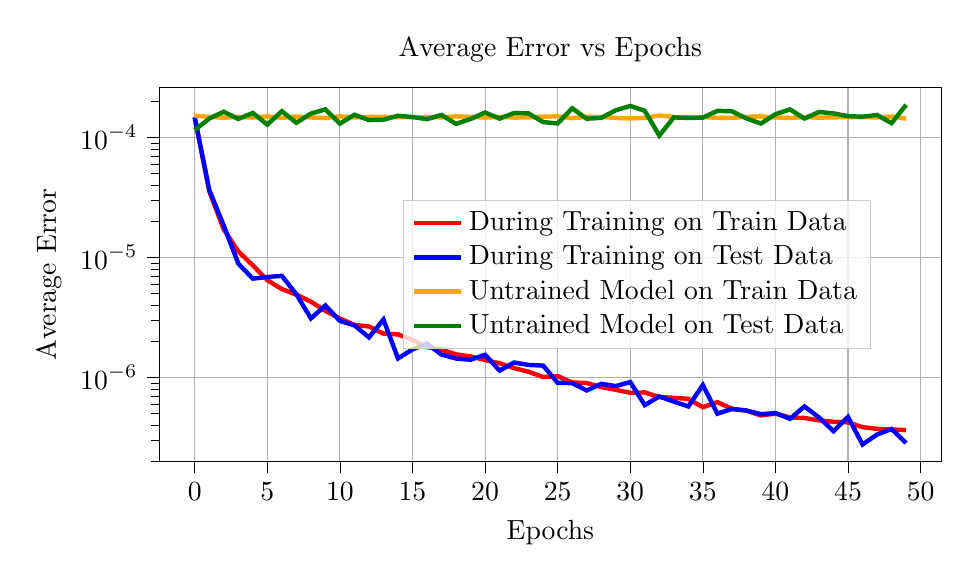
\begin{tikzpicture}

  \definecolor{darkgray176}{RGB}{176,176,176}
  \definecolor{green}{RGB}{0,128,0}
  \definecolor{lightgray204}{RGB}{204,204,204}
  \definecolor{orange}{RGB}{255,165,0}
  
  \begin{axis}[
    width = 0.95\textwidth,
    height = 18em,
  legend cell align={left},
  legend style={
    fill opacity=0.8,
    draw opacity=1,
    text opacity=1,
    at={(0.91,0.5)},
    anchor=east,
    draw=lightgray204
  },
  % log basis y={10},
  tick align=outside,
  tick pos=left,
  title={Average Error vs Epochs},
  x grid style={darkgray176},
  xlabel={Epochs},
  xmajorgrids,
  xmin=-2.45, xmax=51.45,
  xtick style={color=black},
  y grid style={darkgray176},
  ylabel={Average Error},
  ymajorgrids,
  ymin=1.98989848731464e-07, ymax=0.00025862395496495,
  ymode=log,
  ytick style={color=black},
  ytick={1e-08,1e-07,1e-06,1e-05,0.0001,0.001,0.01},
  yticklabels={
    \(\displaystyle {10^{-8}}\),
    \(\displaystyle {10^{-7}}\),
    \(\displaystyle {10^{-6}}\),
    \(\displaystyle {10^{-5}}\),
    \(\displaystyle {10^{-4}}\),
    \(\displaystyle {10^{-3}}\),
    \(\displaystyle {10^{-2}}\)
  }
  ]
  \addplot [ultra thick, red]
  table {%
  0 0.000148013044963591
  1 3.56593227479607e-05
  2 1.7092230336857e-05
  3 1.12235911728931e-05
  4 8.58035764395026e-06
  5 6.45710269964184e-06
  6 5.44462363905041e-06
  7 4.88857358504902e-06
  8 4.2726201172627e-06
  9 3.58169586434087e-06
  10 3.09524739350309e-06
  11 2.73389900939947e-06
  12 2.65521657638601e-06
  13 2.31281637752545e-06
  14 2.27968439503456e-06
  15 2.05286619348044e-06
  16 1.78653704097087e-06
  17 1.69934662608284e-06
  18 1.55517341227096e-06
  19 1.49384698033828e-06
  20 1.3938711163064e-06
  21 1.30992964386678e-06
  22 1.19467654258187e-06
  23 1.11279143766296e-06
  24 1.00586737517006e-06
  25 1.02330841400544e-06
  26 9.0733004753929e-07
  27 8.96316521448171e-07
  28 8.29465079732472e-07
  29 7.87274132107996e-07
  30 7.43528971725027e-07
  31 7.48820809803874e-07
  32 6.85715860981873e-07
  33 6.74960119795287e-07
  34 6.62006982565799e-07
  35 5.64021263471659e-07
  36 6.21000424416707e-07
  37 5.4747005151512e-07
  38 5.2761015467695e-07
  39 4.81172207855707e-07
  40 4.98232964218914e-07
  41 4.6397821051869e-07
  42 4.58541705938842e-07
  43 4.38037005778824e-07
  44 4.26196010039348e-07
  45 4.2150298895649e-07
  46 3.84383071150296e-07
  47 3.72081899513432e-07
  48 3.67385837307665e-07
  49 3.63334208941524e-07
  };
  \addlegendentry{During Training on Train Data}
  \addplot [ultra thick, blue]
  table {%
  0 0.000145961690577678
  1 3.6507273762254e-05
  2 1.83924421435222e-05
  3 8.87434453034075e-06
  4 6.65402694721706e-06
  5 6.85723716742359e-06
  6 7.01677663528244e-06
  7 4.92142953589791e-06
  8 3.10200198327948e-06
  9 3.96965651816572e-06
  10 2.95227073365822e-06
  11 2.71325984613213e-06
  12 2.15284285332018e-06
  13 3.03261163026036e-06
  14 1.43896522786235e-06
  15 1.70873647675762e-06
  16 1.90969149116427e-06
  17 1.54746635416814e-06
  18 1.43470697366865e-06
  19 1.4017372222952e-06
  20 1.54278404806973e-06
  21 1.13814337510121e-06
  22 1.32910520278529e-06
  23 1.26849226944614e-06
  24 1.25276187645795e-06
  25 9.00273789739003e-07
  26 8.95020548341563e-07
  27 7.7743254678353e-07
  28 8.83171367149771e-07
  29 8.45460078835458e-07
  30 9.13137625957461e-07
  31 5.87568308674236e-07
  32 6.92485286890587e-07
  33 6.28680254521896e-07
  34 5.71698194562487e-07
  35 8.63643435877748e-07
  36 4.98133147175395e-07
  37 5.44820807135693e-07
  38 5.29007309069129e-07
  39 4.93094887588086e-07
  40 5.04310378346418e-07
  41 4.50991336720108e-07
  42 5.72123838082916e-07
  43 4.63405569917086e-07
  44 3.56029943304748e-07
  45 4.6835725697747e-07
  46 2.75656987014372e-07
  47 3.33770287852531e-07
  48 3.71070939308993e-07
  49 2.83416682123061e-07
  };
  \addlegendentry{During Training on Test Data}
  \addplot [ultra thick, orange]
  table {%
  0 0.000151286862092093
  1 0.000148271938087419
  2 0.000145962316310033
  3 0.000148140708915889
  4 0.000146270336699672
  5 0.000149768020492047
  6 0.000145538549986668
  7 0.000149274768773466
  8 0.000146568301715888
  9 0.000144949066452682
  10 0.00014968030154705
  11 0.000146915088407695
  12 0.000148198654642329
  13 0.000148643390275538
  14 0.000147157494211569
  15 0.000147706436109729
  16 0.00014777151227463
  17 0.00014694788842462
  18 0.000149669518577866
  19 0.000148425155202858
  20 0.000146184596815147
  21 0.000148376799188554
  22 0.000146324280649424
  23 0.00014655634004157
  24 0.000149089726619422
  25 0.000149657396832481
  26 0.000144709527376108
  27 0.000148061357322149
  28 0.000147991930134594
  29 0.000145307276397943
  30 0.000143848243169487
  31 0.000145373909617774
  32 0.000152415770571679
  33 0.000147752347402275
  34 0.00014776736497879
  35 0.000147837854456156
  36 0.000145569443702698
  37 0.000145633559441194
  38 0.000148161940160207
  39 0.000149608822539449
  40 0.000146714635775425
  41 0.000145101090311073
  42 0.000147954560816288
  43 0.000146047284943052
  44 0.000147063998156227
  45 0.000147197628393769
  46 0.000147608181578107
  47 0.000146761129144579
  48 0.000149398503708653
  49 0.000143366807606071
  };
  \addlegendentry{Untrained Model on Train Data}
  \addplot [ultra thick, green]
  table {%
  0 0.000115061491669621
  1 0.000143547338666394
  2 0.000163512173458003
  3 0.000142517077620141
  4 0.000159814182552509
  5 0.00012783041165676
  6 0.000165362667758018
  7 0.000132426110212691
  8 0.000157876085722819
  9 0.000171300649526529
  10 0.000130172455101274
  11 0.000154473222210072
  12 0.000139474926982075
  13 0.000140412186738104
  14 0.000151597065269016
  15 0.00014767273387406
  16 0.000141933254781179
  17 0.000153813511133194
  18 0.000129606123664416
  19 0.000142261982546188
  20 0.000161294257850386
  21 0.00014334442676045
  22 0.000159681003424339
  23 0.000158348615514114
  24 0.000134108049678616
  25 0.000130705229821615
  26 0.000174892600625753
  27 0.000143100725836121
  28 0.000145519719808362
  29 0.000168184196809307
  30 0.000182958712684922
  31 0.000166574260219932
  32 0.000103557540569454
  33 0.000146681413752958
  34 0.000145311874803156
  35 0.00014605671458412
  36 0.000166460915352218
  37 0.000165033299708739
  38 0.000144075253047049
  39 0.000130360465846024
  40 0.000155840680235997
  41 0.000171156978467479
  42 0.000143605619086884
  43 0.000162815587827936
  44 0.000158585360622965
  45 0.000150236810441129
  46 0.000148762876051478
  47 0.000153807501192205
  48 0.000131454333313741
  49 0.000186694131116383
  };
  \addlegendentry{Untrained Model on Test Data}
  \end{axis}
  
  \end{tikzpicture}
  
%   % \end{turn}
%   \caption{URWF scenario $7$, layers$=10$, epochs$=50$, learning rate$=10^{-3}$}
%     % \label{fig:wf_dfghvariants}
%   \end{figure}
% %   \clearpage % End the page
% }



\afterpage{%
%   \clearpage % Start a new page
\begin{figure}[!htbp]
  \subfloat[First Scenario: Single Scalar$(\tau)$]{% This file was created with tikzplotlib v0.10.1.
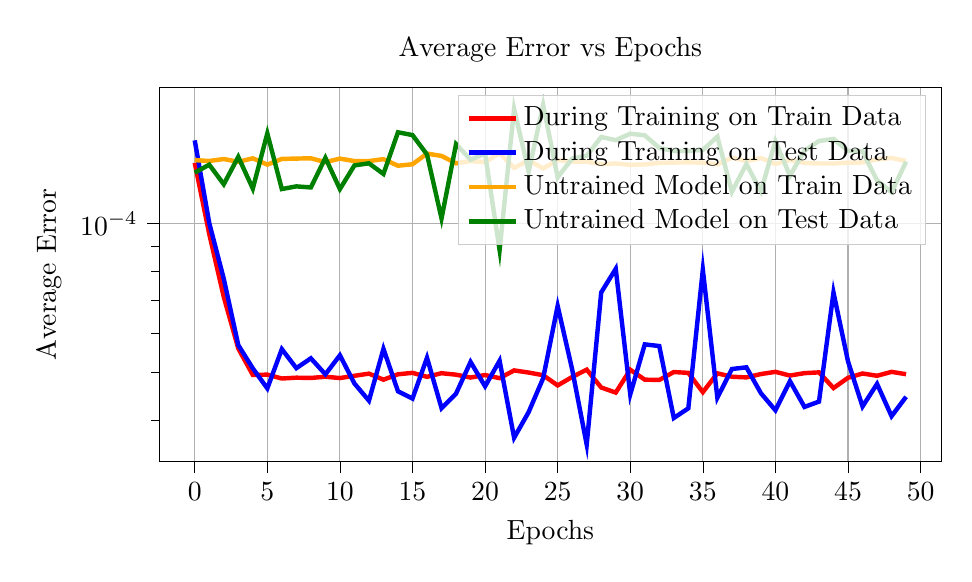
\begin{tikzpicture}

  \definecolor{darkgray176}{RGB}{176,176,176}
  \definecolor{green}{RGB}{0,128,0}
  \definecolor{lightgray204}{RGB}{204,204,204}
  \definecolor{orange}{RGB}{255,165,0}
  
  \begin{axis}[
    width = 0.95\textwidth,
    height = 18em,
  legend cell align={left},
  legend style={
    fill opacity=0.8,
    draw opacity=1,
    text opacity=1,
    % at={(0.91,0.5)},
    % anchor=east,
    draw=lightgray204
  },
  % log basis y={10},
  tick align=outside,
  tick pos=left,
  title={Average Error vs Epochs},
  x grid style={darkgray176},
  xlabel={Epochs},
  xmajorgrids,
  xmin=-2.45, xmax=51.45,
  xtick style={color=black},
  y grid style={darkgray176},
  ylabel={Average Error},
  ymajorgrids,
  ymin=3.30722135247185e-05, ymax=0.000188104234714924,
  ymode=log,
  ytick style={color=black},
  ytick={1e-06,1e-05,0.0001,0.001,0.01},
  yticklabels={
    \(\displaystyle {10^{-6}}\),
    \(\displaystyle {10^{-5}}\),
    \(\displaystyle {10^{-4}}\),
    \(\displaystyle {10^{-3}}\),
    \(\displaystyle {10^{-2}}\)
  }
  ]
  \addplot [ultra thick, red]
  table {%
  0 0.000132722096168436
  1 9.52958143898286e-05
  2 7.11312095518224e-05
  3 5.59525251446757e-05
  4 4.94734194944613e-05
  5 4.95356325700413e-05
  6 4.86540520796552e-05
  7 4.88426849187817e-05
  8 4.87789220642298e-05
  9 4.90620986965951e-05
  10 4.87564029754139e-05
  11 4.92705366923474e-05
  12 4.97732726216782e-05
  13 4.83878284285311e-05
  14 4.96224929520395e-05
  15 4.99510824738536e-05
  16 4.90340717078652e-05
  17 4.98722329211887e-05
  18 4.95317617605906e-05
  19 4.88754849357065e-05
  20 4.94462146889418e-05
  21 4.87317229271866e-05
  22 5.05235257151071e-05
  23 5.0024245865643e-05
  24 4.94094638270326e-05
  25 4.71192179247737e-05
  26 4.90080456074793e-05
  27 5.07079239469022e-05
  28 4.66571473225486e-05
  29 4.55734552815557e-05
  30 5.06827636854723e-05
  31 4.83968869957607e-05
  32 4.83256881125271e-05
  33 5.0144979468314e-05
  34 4.99464476888534e-05
  35 4.56594752904493e-05
  36 4.98443841934204e-05
  37 4.90569836983923e-05
  38 4.89077756355982e-05
  39 4.96737193316221e-05
  40 5.01869035360869e-05
  41 4.93312109028921e-05
  42 4.98860681545921e-05
  43 5.00653732160572e-05
  44 4.65431585325859e-05
  45 4.88188707095105e-05
  46 4.98049921588972e-05
  47 4.92811013828032e-05
  48 5.01822796650231e-05
  49 4.96389002364594e-05
  };
  \addlegendentry{During Training on Train Data}
  \addplot [ultra thick, blue]
  table {%
  0 0.000147356346133165
  1 0.000100276833109092
  2 7.74033032939769e-05
  3 5.68429713894147e-05
  4 5.10137870151084e-05
  5 4.64688382635359e-05
  6 5.57806524739135e-05
  7 5.1057828386547e-05
  8 5.34521313966252e-05
  9 4.96142783958931e-05
  10 5.42103043699171e-05
  11 4.7545585402986e-05
  12 4.38857059634756e-05
  13 5.58492865820881e-05
  14 4.58449612779077e-05
  15 4.43196513515431e-05
  16 5.35876279172953e-05
  17 4.23945093643852e-05
  18 4.53545399068389e-05
  19 5.25535251654219e-05
  20 4.69236656499561e-05
  21 5.28460477653425e-05
  22 3.69406589015853e-05
  23 4.16071488871239e-05
  24 4.87198121845722e-05
  25 6.8199158704374e-05
  26 5.0729689974105e-05
  27 3.57913850166369e-05
  28 7.26350262993947e-05
  29 8.1043537647929e-05
  30 4.51905725640245e-05
  31 5.70314368815161e-05
  32 5.65893242310267e-05
  33 4.04946149501484e-05
  34 4.23562341893557e-05
  35 8.07066462584771e-05
  36 4.44882716692518e-05
  37 5.08558587171137e-05
  38 5.12504157086369e-05
  39 4.54418550361879e-05
  40 4.19671923737042e-05
  41 4.80627386423294e-05
  42 4.26279038947541e-05
  43 4.37011694884859e-05
  44 7.25988211343065e-05
  45 5.26790354342666e-05
  46 4.27131417382043e-05
  47 4.74478620162699e-05
  48 4.08320811402518e-05
  49 4.46896556240972e-05
  };
  \addlegendentry{During Training on Test Data}
  \addplot [ultra thick, orange]
  table {%
  0 0.000134415182401426
  1 0.000133859735797159
  2 0.000135096372105181
  3 0.000133315537823364
  4 0.000135558802867308
  5 0.000131604872876778
  6 0.000135166221298277
  7 0.000135371694341302
  8 0.00013555760961026
  9 0.000133147303131409
  10 0.000135355425300077
  11 0.000133816851302981
  12 0.00013382603356149
  13 0.000135015754494816
  14 0.000130949250888079
  15 0.000131850087200291
  16 0.000138567527756095
  17 0.000137042501592077
  18 0.000132412038510665
  19 0.000133806184749119
  20 0.00013315056276042
  21 0.000138728239107877
  22 0.000129598542116582
  23 0.000134296817122959
  24 0.000129316467791796
  25 0.000134426998556592
  26 0.000133511028252542
  27 0.000133338689920492
  28 0.000131890992633998
  29 0.000132342014694586
  30 0.000131475171656348
  31 0.000131742417579517
  32 0.000132709450554103
  33 0.000132882501929998
  34 0.000132975561427884
  35 0.0001328465732513
  36 0.000131782973767258
  37 0.000135892565594986
  38 0.000133842084323987
  39 0.000135688576847315
  40 0.000132072207634337
  41 0.000134420246467926
  42 0.000132650457089767
  43 0.000132311062770896
  44 0.000132282293634489
  45 0.000132839733851142
  46 0.00013292086077854
  47 0.00013482163194567
  48 0.000135752008645795
  49 0.000133861845824867
  };
  \addlegendentry{Untrained Model on Train Data}
  \addplot [ultra thick, green]
  table {%
  0 0.00012677519407589
  1 0.000131578868604265
  2 0.000120126052934211
  3 0.000136456466862001
  4 0.000117726136522833
  5 0.000152216060087085
  6 0.000117487055831589
  7 0.000118944961286616
  8 0.000118362011562567
  9 0.000135828202473931
  10 0.000117471114208456
  11 0.000131132823298685
  12 0.0001324288896285
  13 0.00012603857612703
  14 0.000153000306454487
  15 0.000151011321577244
  16 0.000137982569867745
  17 0.000102457801403943
  18 0.000144789562909864
  19 0.0001346626522718
  20 0.00013855162251275
  21 8.84784312802367e-05
  22 0.000170658269780688
  23 0.000127359642647207
  24 0.000173813430592418
  25 0.000124067300930619
  26 0.000135398469865322
  27 0.000137087437906303
  28 0.00014967487368267
  29 0.000147490325616673
  30 0.000151992935570888
  31 0.000150832158396952
  32 0.000142279764986597
  33 0.000140183008625172
  34 0.000140295756864361
  35 0.000140935080708005
  36 0.000149868414155208
  37 0.000115996052045375
  38 0.000131940701976418
  39 0.000116244016680866
  40 0.000146826612763107
  41 0.000124963815324008
  42 0.000140456089866348
  43 0.000146886712173
  44 0.000148353181430139
  45 0.000140342046506703
  46 0.000139979019877501
  47 0.000122307494166307
  48 0.000115747614472639
  49 0.000133389243273996
  };
  \addlegendentry{Untrained Model on Test Data}
  \end{axis}
  
  \end{tikzpicture}
  }\\
  \subfloat[Second Scenario: Different Scalars$(\tau_k)$]{% This file was created with tikzplotlib v0.10.1.
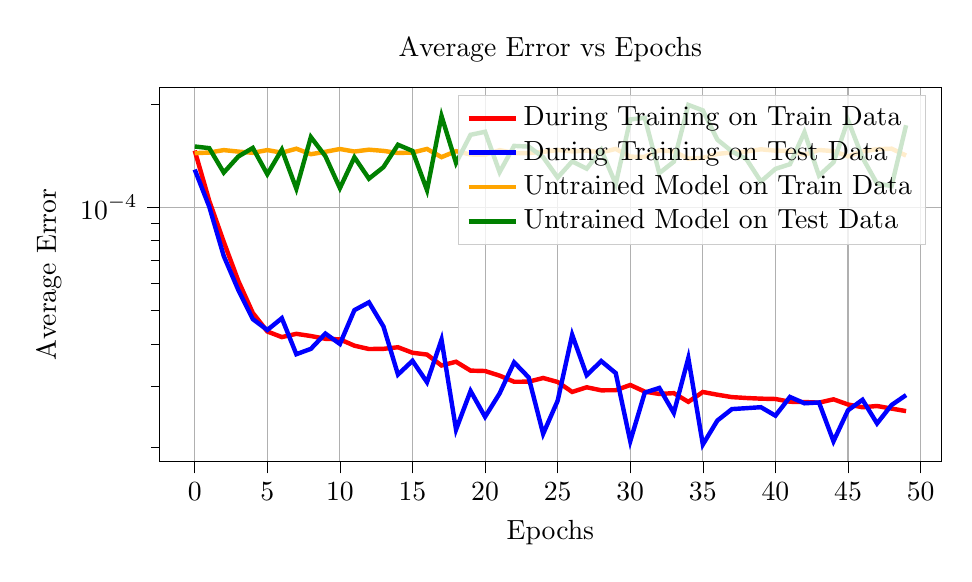
\begin{tikzpicture}

    \definecolor{darkgray176}{RGB}{176,176,176}
    \definecolor{green}{RGB}{0,128,0}
    \definecolor{lightgray204}{RGB}{204,204,204}
    \definecolor{orange}{RGB}{255,165,0}
    
    \begin{axis}[
      width = 0.95\textwidth,
      height = 18em,
    legend cell align={left},
    legend style={
      fill opacity=0.8,
      draw opacity=1,
      text opacity=1,
      % at={(0.91,0.5)},
      % anchor=east,
      draw=lightgray204
    },
    % log basis y={10},
    tick align=outside,
    tick pos=left,
    title={Average Error vs Epochs},
    x grid style={darkgray176},
    xlabel={Epochs},
    xmajorgrids,
    xmin=-2.45, xmax=51.45,
    xtick style={color=black},
    y grid style={darkgray176},
    ylabel={Average Error},
    ymajorgrids,
    ymin=1.81602095355054e-05, ymax=0.000222783350611656,
    ymode=log,
    ytick style={color=black},
    ytick={1e-06,1e-05,0.0001,0.001,0.01},
    yticklabels={
      \(\displaystyle {10^{-6}}\),
      \(\displaystyle {10^{-5}}\),
      \(\displaystyle {10^{-4}}\),
      \(\displaystyle {10^{-3}}\),
      \(\displaystyle {10^{-2}}\)
    }
    ]
    \addplot [ultra thick, red]
    table {%
    0 0.000146278194733895
    1 0.000104420905699953
    2 7.92681239545345e-05
    3 6.10758288530633e-05
    4 4.92224680783693e-05
    5 4.34550092904828e-05
    6 4.18473209720105e-05
    7 4.27740997110959e-05
    8 4.21492586610839e-05
    9 4.13740053772926e-05
    10 4.12062763643917e-05
    11 3.95096503780223e-05
    12 3.86323808925226e-05
    13 3.8685386243742e-05
    14 3.90951099689119e-05
    15 3.7674093618989e-05
    16 3.72231625078712e-05
    17 3.45841617672704e-05
    18 3.54710755345877e-05
    19 3.34202304657083e-05
    20 3.33290299749933e-05
    21 3.23112872138154e-05
    22 3.10100913338829e-05
    23 3.1028324883664e-05
    24 3.18035745294765e-05
    25 3.09636925521772e-05
    26 2.89666477328865e-05
    27 2.98817540169694e-05
    28 2.92815784632694e-05
    29 2.92987824650481e-05
    30 3.03483375319047e-05
    31 2.90223379124654e-05
    32 2.85742298729019e-05
    33 2.87294860754628e-05
    34 2.71037642960437e-05
    35 2.89524341496872e-05
    36 2.84268226096174e-05
    37 2.79751275229501e-05
    38 2.78087027254514e-05
    39 2.76841983577469e-05
    40 2.76240880339174e-05
    41 2.71164917649003e-05
    42 2.70670807367424e-05
    43 2.69537595158909e-05
    44 2.75629245152231e-05
    45 2.6622759833117e-05
    46 2.61352506640833e-05
    47 2.63559304585215e-05
    48 2.59002445091028e-05
    49 2.54677142947912e-05
    };
    \addlegendentry{During Training on Train Data}
    \addplot [ultra thick, blue]
    table {%
    0 0.000128779443912208
    1 0.00010038409527624
    2 7.20859316061251e-05
    3 5.74429686821532e-05
    4 4.72210740554146e-05
    5 4.38880924775731e-05
    6 4.74986336485017e-05
    7 3.7310368497856e-05
    8 3.86739084206056e-05
    9 4.2848852899624e-05
    10 3.9968599594431e-05
    11 5.0143735279562e-05
    12 5.285011138767e-05
    13 4.49300969194155e-05
    14 3.25484543282073e-05
    15 3.56887139787432e-05
    16 3.09173701680265e-05
    17 4.11355395044666e-05
    18 2.24964205699507e-05
    19 2.91467531496892e-05
    20 2.45067039941205e-05
    21 2.86695176328067e-05
    22 3.53258474206086e-05
    23 3.19383507303428e-05
    24 2.18671866605291e-05
    25 2.73038804152748e-05
    26 4.2485826270422e-05
    27 3.24111788359005e-05
    28 3.56320124410558e-05
    29 3.28617716149893e-05
    30 2.08107903745258e-05
    31 2.8820493753301e-05
    32 2.97523602057481e-05
    33 2.5161634766846e-05
    34 3.63602011930197e-05
    35 2.03521376533899e-05
    36 2.3903059627628e-05
    37 2.58119016507408e-05
    38 2.59747375821462e-05
    39 2.61434706771979e-05
    40 2.47025800490519e-05
    41 2.80039475910598e-05
    42 2.68369312834693e-05
    43 2.69887150352588e-05
    44 2.07989851332968e-05
    45 2.56072144111386e-05
    46 2.74763297056779e-05
    47 2.34442468354246e-05
    48 2.65273101831554e-05
    49 2.83582612610189e-05
    };
    \addlegendentry{During Training on Test Data}
    \addplot [ultra thick, orange]
    table {%
    0 0.000143817727803253
    1 0.000144362973514944
    2 0.000146766687976196
    3 0.000145289624924771
    4 0.000144115459988825
    5 0.000146782738738693
    6 0.000144232981256209
    7 0.000148136517964303
    8 0.000142785676871426
    9 0.000145113124744967
    10 0.000147847051266581
    11 0.000145348269143142
    12 0.000147180369822308
    13 0.000145986239658669
    14 0.000143930912599899
    15 0.000144404504681006
    16 0.000147901533637196
    17 0.000139990574098192
    18 0.000145746729685925
    19 0.000142500211950392
    20 0.000142163597047329
    21 0.000146696082083508
    22 0.00014386406110134
    23 0.000143894605571404
    24 0.000145068916026503
    25 0.000146825681440532
    26 0.000145544589031488
    27 0.000146261707413942
    28 0.000144508856465109
    29 0.000147926708450541
    30 0.000140387055580504
    31 0.000140381875098683
    32 0.00014663758338429
    33 0.00014546888996847
    34 0.000138474060804583
    35 0.000139353855047375
    36 0.000143018041853793
    37 0.000144513905979693
    38 0.000145408208481967
    39 0.00014754910080228
    40 0.000146216785651632
    41 0.000146020873216912
    42 0.000142244753078558
    43 0.000146861115354113
    44 0.000145769605296664
    45 0.000140737523906864
    46 0.000145486628753133
    47 0.000147612619912252
    48 0.000148156919749454
    49 0.000141483877087012
    };
    \addlegendentry{Untrained Model on Train Data}
    \addplot [ultra thick, green]
    table {%
    0 0.000150364750879817
    1 0.000148715800605714
    2 0.000126212136819959
    3 0.000140571341034956
    4 0.00014891754835844
    5 0.0001248148328159
    6 0.000147257611388341
    7 0.000113281806989107
    8 0.000160188879817724
    9 0.000140890551847406
    10 0.000113709320430644
    11 0.000139861251227558
    12 0.00012114318087697
    13 0.000130904605612159
    14 0.000152134743984789
    15 0.000145973521284759
    16 0.000112183719465975
    17 0.000184424745384604
    18 0.000134632413391955
    19 0.00016261384007521
    20 0.000165981182362884
    21 0.00012655348109547
    22 0.000150970416143537
    23 0.000150248713907786
    24 0.000139949814183637
    25 0.000122067860502284
    26 0.000136034286697395
    27 0.000129538966575637
    28 0.000146950769703835
    29 0.000116940143925603
    30 0.000180271337740123
    31 0.000182227056939155
    32 0.000125736318295822
    33 0.000135748166940175
    34 0.000198789552086964
    35 0.000191611266927794
    36 0.000157448623212986
    37 0.000145551850437187
    38 0.000138119357870892
    39 0.000118853095045779
    40 0.000129383552120999
    41 0.000133493827888742
    42 0.00016541252261959
    43 0.000123607329442166
    44 0.000135195485199802
    45 0.000179384034709074
    46 0.000139412193675525
    47 0.00011720007751137
    48 0.000115313268906903
    49 0.000173394801095128
    };
    \addlegendentry{Untrained Model on Test Data}
    \end{axis}
    
    \end{tikzpicture}
    }\\
  \subfloat[Third Scenario: Single Matrix$(\boldsymbol{M})$]{% This file was created with tikzplotlib v0.10.1.
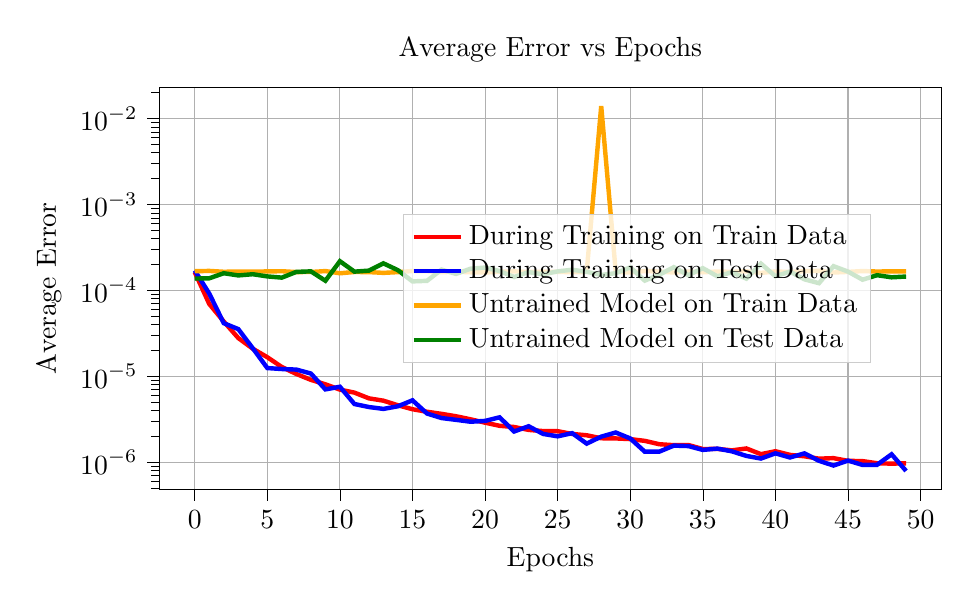
\begin{tikzpicture}

  \definecolor{darkgray176}{RGB}{176,176,176}
  \definecolor{green}{RGB}{0,128,0}
  \definecolor{lightgray204}{RGB}{204,204,204}
  \definecolor{orange}{RGB}{255,165,0}
  
  \begin{axis}[
    width = 0.95\textwidth,
    height = 19em,
  legend cell align={left},
  legend style={
    fill opacity=0.8,
    draw opacity=1,
    text opacity=1,
    at={(0.91,0.5)},
    anchor=east,
    draw=lightgray204
  },
  % log basis y={10},
  tick align=outside,
  tick pos=left,
  title={Average Error vs Epochs},
  x grid style={darkgray176},
  xlabel={Epochs},
  xmajorgrids,
  xmin=-2.45, xmax=51.45,
  xtick style={color=black},
  y grid style={darkgray176},
  ylabel={Average Error},
  ymajorgrids,
  ymin=4.86653883990184e-07, ymax=0.0227388191398161,
  ymode=log,
  ytick style={color=black},
  ytick={1e-08,1e-07,1e-06,1e-05,0.0001,0.001,0.01,0.1,1},
yticklabels={
  \(\displaystyle {10^{-8}}\),
  \(\displaystyle {10^{-7}}\),
  \(\displaystyle {10^{-6}}\),
  \(\displaystyle {10^{-5}}\),
  \(\displaystyle {10^{-4}}\),
  \(\displaystyle {10^{-3}}\),
  \(\displaystyle {10^{-2}}\),
  \(\displaystyle {10^{-1}}\),
  \(\displaystyle {10^{0}}\)
}
  ]
  \addplot [ultra thick, red]
table {%
0 0.000163097938639112
1 6.95640046615154e-05
2 4.34557296102867e-05
3 2.79197738564108e-05
4 2.09615609492175e-05
5 1.66988993441919e-05
6 1.28378760564374e-05
7 1.0652799574018e-05
8 9.10444123292109e-06
9 8.07891319709597e-06
10 7.00679311194108e-06
11 6.46568105366896e-06
12 5.54613734493614e-06
13 5.20814501214772e-06
14 4.60338424090878e-06
15 4.14187388741993e-06
16 3.87155705539044e-06
17 3.66023209608102e-06
18 3.43169858751935e-06
19 3.16300565827987e-06
20 2.88951900984102e-06
21 2.65776702690346e-06
22 2.57361512012722e-06
23 2.38001484831329e-06
24 2.30703153647482e-06
25 2.29981696975301e-06
26 2.13718476516078e-06
27 2.06161598725885e-06
28 1.90302205282933e-06
29 1.89487604984606e-06
30 1.86091483556083e-06
31 1.7752225858203e-06
32 1.62237029144308e-06
33 1.58172042574733e-06
34 1.58960199314606e-06
35 1.42605972541787e-06
36 1.43255817874888e-06
37 1.37571066716191e-06
38 1.44837963489408e-06
39 1.24299731396604e-06
40 1.34513811644865e-06
41 1.21901894090115e-06
42 1.17452839276666e-06
43 1.10200176095532e-06
44 1.11689780624147e-06
45 1.03926151950873e-06
46 1.03192769529414e-06
47 9.74933186626004e-07
48 9.63614297688764e-07
49 9.73476744547952e-07
};
\addlegendentry{During Training on Train Data}
\addplot [ultra thick, blue]
table {%
0 0.000170692641404457
1 9.19459635042585e-05
2 4.15414688177407e-05
3 3.54702751792502e-05
4 2.12094691960374e-05
5 1.24855350804864e-05
6 1.21629809655133e-05
7 1.19845199151314e-05
8 1.07882378870272e-05
9 7.0505338953808e-06
10 7.56783765609725e-06
11 4.76404329674551e-06
12 4.39399946117192e-06
13 4.18000399804441e-06
14 4.48639048045152e-06
15 5.26103758602403e-06
16 3.69247027265374e-06
17 3.27280577039346e-06
18 3.11769122163241e-06
19 2.96365715257707e-06
20 3.03114143207495e-06
21 3.33551702169643e-06
22 2.28128169510455e-06
23 2.62626690528123e-06
24 2.1363327959989e-06
25 2.00401018446428e-06
26 2.18199670598551e-06
27 1.64860466611572e-06
28 1.9884250832547e-06
29 2.22067751565191e-06
30 1.89409990980494e-06
31 1.32749971726298e-06
32 1.33019966597203e-06
33 1.56249666360964e-06
34 1.54365932303335e-06
35 1.39256223974371e-06
36 1.44203693253075e-06
37 1.34115566652326e-06
38 1.18524599201919e-06
39 1.10521705209976e-06
40 1.27091846024996e-06
41 1.1371939763194e-06
42 1.26946542877704e-06
43 1.04059097338904e-06
44 9.16003955353517e-07
45 1.04647676835157e-06
46 9.31057911657263e-07
47 9.34875686198211e-07
48 1.23812992569583e-06
49 7.93363767570554e-07
};
\addlegendentry{During Training on Test Data}
\addplot [ultra thick, orange]
table {%
0 0.000167268663062714
1 0.000168611761182547
2 0.000164750032126904
3 0.000166074707522057
4 0.000165510311489925
5 0.000166329540661536
6 0.000167264486663043
7 0.000163467208039947
8 0.000163789329235442
9 0.000167902631801553
10 0.000158251743414439
11 0.000163772841915488
12 0.000163379823789001
13 0.000159947972861119
14 0.000163212345796637
15 0.000168250291608274
16 0.000167275851708837
17 0.00016272951324936
18 0.000165133300470188
19 0.000162475116667338
20 0.000161717063747346
21 0.000164484881679527
22 0.000166474826983176
23 0.000163901393534616
24 0.00016524524835404
25 0.000164450189913623
26 0.000162684242241085
27 0.000163810182129964
28 0.0139481220394373
29 0.00016462522034999
30 0.000161635733093135
31 0.000168101963936351
32 0.000165689591085538
33 0.000161484422278591
34 0.000165562189067714
35 0.000162491676746868
36 0.000165928257047199
37 0.000164456811035052
38 0.000166921367053874
39 0.000159998307935894
40 0.000166102094226517
41 0.000163806194905192
42 0.000167545396834612
43 0.000168941318406723
44 0.000161504111019894
45 0.000164178913109936
46 0.000167981517734006
47 0.000165818899404258
48 0.000166785175679252
49 0.000166209385497496
};
\addlegendentry{Untrained Model on Train Data}
\addplot [ultra thick, green]
table {%
0 0.000137429335154593
1 0.000138295567012392
2 0.000158476585056633
3 0.000149381274241023
4 0.000154329158249311
5 0.000145530575537123
6 0.000140856049256399
7 0.000164252924150787
8 0.000166630212333985
9 0.000129618609207682
10 0.000218662316910923
11 0.000165390243637376
12 0.000169930906849913
13 0.000206377269933
14 0.00017179134010803
15 0.000127295410493389
16 0.000129273044876754
17 0.000174764529219829
18 0.000155563189764507
19 0.00017893330368679
20 0.00018444396846462
21 0.000167917532962747
22 0.000143270124681294
23 0.000163351345690899
24 0.000153900356963277
25 0.000166609228472225
26 0.000174030355992727
27 0.000164638928254135
28 0.000151140950038098
29 0.000158716487931088
30 0.000185446187970228
31 0.000130001790239476
32 0.000152179549331777
33 0.000186295816092752
34 0.000150395178934559
35 0.000181550378329121
36 0.000145733851240948
37 0.000162864715093747
38 0.00013712968211621
39 0.000205252305022441
40 0.000145977654028684
41 0.000165515957633033
42 0.000134605827042833
43 0.000121332785056438
44 0.00019154827168677
45 0.000165487450431101
46 0.00013320310972631
47 0.000150331645272672
48 0.000142030883580446
49 0.000145056197652593
};
\addlegendentry{Untrained Model on Test Data}
\end{axis}

\end{tikzpicture}}\\  
  \caption{Training the \ac{RWF} Algorithm in different Scenarios}
  \label{some examsdafple}
  \end{figure}

%   \clearpage % End the page
}
\afterpage{%
%   \clearpage % Start a new page
\begin{figure}[!htbp]
  \subfloat[Fourth Scenario: Single Semi-Positive Definite Matrix$(\boldsymbol{S})$]{% This file was created with tikzplotlib v0.10.1.
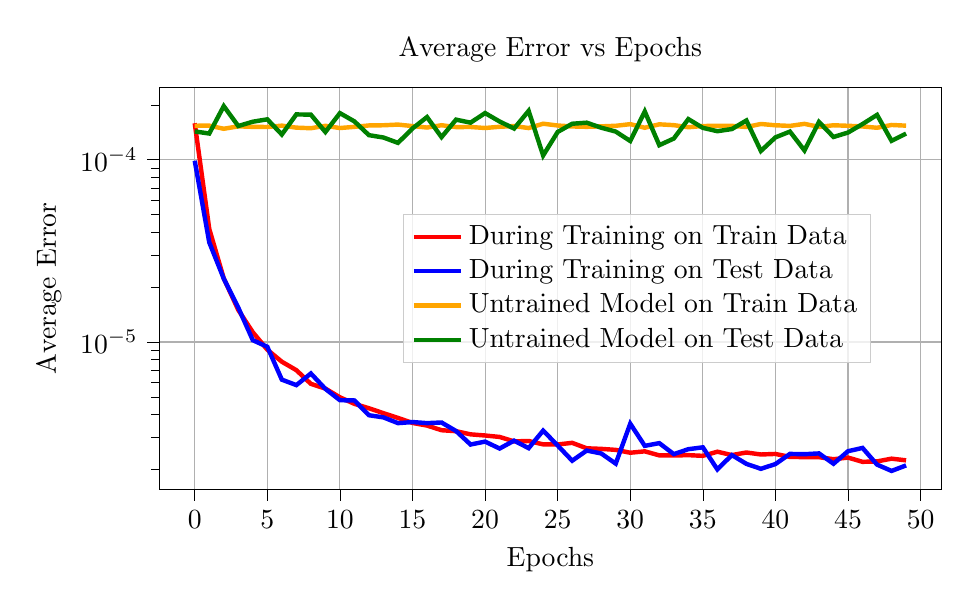
\begin{tikzpicture}

  \definecolor{darkgray176}{RGB}{176,176,176}
  \definecolor{green}{RGB}{0,128,0}
  \definecolor{lightgray204}{RGB}{204,204,204}
  \definecolor{orange}{RGB}{255,165,0}
  
  \begin{axis}[
    width = 0.95\textwidth,
    height = 19em,
  legend cell align={left},
  legend style={
    fill opacity=0.8,
    draw opacity=1,
    text opacity=1,
    at={(0.91,0.5)},
    anchor=east,
    draw=lightgray204
  },
  % log basis y={10},
  tick align=outside,
  tick pos=left,
  title={Average Error vs Epochs},
  x grid style={darkgray176},
  xlabel={Epochs},
  xmajorgrids,
  xmin=-2.45, xmax=51.45,
  xtick style={color=black},
  y grid style={darkgray176},
  ylabel={Average Error},
  ymajorgrids,
  ymin=1.55984612605889e-06, ymax=0.000247681245738091,
ymode=log,
ytick style={color=black},
ytick={1e-07,1e-06,1e-05,0.0001,0.001,0.01},
yticklabels={
  \(\displaystyle {10^{-7}}\),
  \(\displaystyle {10^{-6}}\),
  \(\displaystyle {10^{-5}}\),
  \(\displaystyle {10^{-4}}\),
  \(\displaystyle {10^{-3}}\),
  \(\displaystyle {10^{-2}}\)
}
  ]
  \addplot [ultra thick, red]
table {%
0 0.000158629423822276
1 4.17500705225393e-05
2 2.23410734179197e-05
3 1.49923098433646e-05
4 1.13186724775005e-05
5 9.07615412870655e-06
6 7.79907350079156e-06
7 7.01064618624514e-06
8 5.89603132539196e-06
9 5.5544014685438e-06
10 4.97701785207028e-06
11 4.58103113487596e-06
12 4.33344484918052e-06
13 4.07163042837055e-06
14 3.83643191526062e-06
15 3.59927594217879e-06
16 3.48308049069601e-06
17 3.28366763824306e-06
18 3.24376105709234e-06
19 3.11671965391724e-06
20 3.07204231830838e-06
21 3.01650766232342e-06
22 2.8517763439595e-06
23 2.86554063677613e-06
24 2.74647231890413e-06
25 2.74263447863632e-06
26 2.79981736639456e-06
27 2.61375680565834e-06
28 2.59432090388145e-06
29 2.56180942415085e-06
30 2.47075331571978e-06
31 2.5146134703391e-06
32 2.38996767620847e-06
33 2.38629627347109e-06
34 2.39670816881699e-06
35 2.37572703554179e-06
36 2.50309471994115e-06
37 2.3985255666048e-06
38 2.47841694545059e-06
39 2.41662883126992e-06
40 2.43350336859294e-06
41 2.34371736951289e-06
42 2.33795276471938e-06
43 2.33626451517921e-06
44 2.27647865358449e-06
45 2.32412526202097e-06
46 2.20256538341346e-06
47 2.21448135562241e-06
48 2.2928848011361e-06
49 2.24423251893313e-06
};
\addlegendentry{During Training on Train Data}
\addplot [ultra thick, blue]
table {%
0 9.87597886705771e-05
1 3.5224966268288e-05
2 2.22798680624692e-05
3 1.54417248268146e-05
4 1.02357944342657e-05
5 9.41831694944995e-06
6 6.21941171630169e-06
7 5.80472351430217e-06
8 6.72237501930795e-06
9 5.53433847017004e-06
10 4.79677191833616e-06
11 4.78111951451865e-06
12 3.96789118894958e-06
13 3.8617140489805e-06
14 3.59103978553321e-06
15 3.64064408131526e-06
16 3.59160890184285e-06
17 3.62066725756449e-06
18 3.25107043863682e-06
19 2.74062654170848e-06
20 2.84425550489686e-06
21 2.60542879004788e-06
22 2.87777834273584e-06
23 2.617919108161e-06
24 3.26798544847406e-06
25 2.70756140707817e-06
26 2.23450524572399e-06
27 2.53932171290217e-06
28 2.44782427216705e-06
29 2.15366708289366e-06
30 3.5666532767209e-06
31 2.6958002763422e-06
32 2.78928996522154e-06
33 2.4274806946778e-06
34 2.58378622675082e-06
35 2.64566619989637e-06
36 2.00250156012771e-06
37 2.39911287280847e-06
38 2.14669603337825e-06
39 2.01651187126117e-06
40 2.1419243694254e-06
41 2.43437216340681e-06
42 2.42601004174503e-06
43 2.44980583374854e-06
44 2.15043269236048e-06
45 2.5189995085384e-06
46 2.62520006799605e-06
47 2.1261782876536e-06
48 1.96389669326891e-06
49 2.10574557968357e-06
};
\addlegendentry{During Training on Test Data}
\addplot [ultra thick, orange]
table {%
0 0.000153553526615724
1 0.0001537842763355
2 0.000147777231177315
3 0.00015241838991642
4 0.00015136860019993
5 0.00015115799033083
6 0.000153794055222534
7 0.000149910119944252
8 0.000148827923112549
9 0.000153429486090317
10 0.000149183717439882
11 0.000151428583194502
12 0.000154140201630071
13 0.000154504115926102
14 0.000155849425937049
15 0.000152900945977308
16 0.000150118707097135
17 0.000154557346832007
18 0.000150987645611167
19 0.00015114396228455
20 0.000149241168401204
21 0.000151554413605481
22 0.00015294119657483
23 0.000149149796925485
24 0.00015752662147861
25 0.000154035544255748
26 0.000152168999193236
27 0.000151451749843545
28 0.000152411332237534
29 0.000153456567204557
30 0.000156663649249822
31 0.000149743806105107
32 0.000156316513312049
33 0.000154719615238719
34 0.000150691892486066
35 0.000153021101141348
36 0.000153451750520617
37 0.000153334884089418
38 0.000151146596181206
39 0.000157007118104957
40 0.000154453708091751
41 0.000153273300384171
42 0.000157264556037262
43 0.000151349857333116
44 0.000154477093019523
45 0.000153465225594118
46 0.000152173946844414
47 0.000149670915561728
48 0.000155075787915848
49 0.000153709916048683
};
\addlegendentry{Untrained Model on Train Data}
\addplot [ultra thick, green]
table {%
0 0.000142935779877007
1 0.000139173978823237
2 0.000196723500266671
3 0.00015302310930565
4 0.000161568226758391
5 0.000166518264450133
6 0.000137492650537752
7 0.000177166191861033
8 0.000176630361238495
9 0.000141880940645933
10 0.000180077680852264
11 0.000162175492732786
12 0.000136325703351758
13 0.000132341476273723
14 0.000123682111734524
15 0.000148397040902637
16 0.00017129372281488
17 0.00013302119623404
18 0.000165837176609784
19 0.000159636896569282
20 0.000180231349077076
21 0.000162036085384898
22 0.000148200779221952
23 0.000185301920282654
24 0.000105486673419364
25 0.000141921264003031
26 0.000157471571583301
27 0.000159628689289093
28 0.000149803585372865
29 0.000142626580782235
30 0.000126621496747248
31 0.000183925643796101
32 0.000120122444059234
33 0.000130652289954014
34 0.000166988946148194
35 0.000149514860822819
36 0.000143318276968785
37 0.000147275306517258
38 0.000164102355483919
39 0.000111702123831492
40 0.000132550703710876
41 0.000142650460475124
42 0.000112421752419323
43 0.000161090036272071
44 0.000133249923237599
45 0.000140913631184958
46 0.000156887806952
47 0.000176143701537512
48 0.000126888087834232
49 0.000139085881528445
};
\addlegendentry{Untrained Model on Test Data}
\end{axis}

\end{tikzpicture}
}\\
  \subfloat[Fifth Scenario: Different Scalars Plus a Single Matrix$(\tau_k\boldsymbol{M})$]{% This file was created with tikzplotlib v0.10.1.
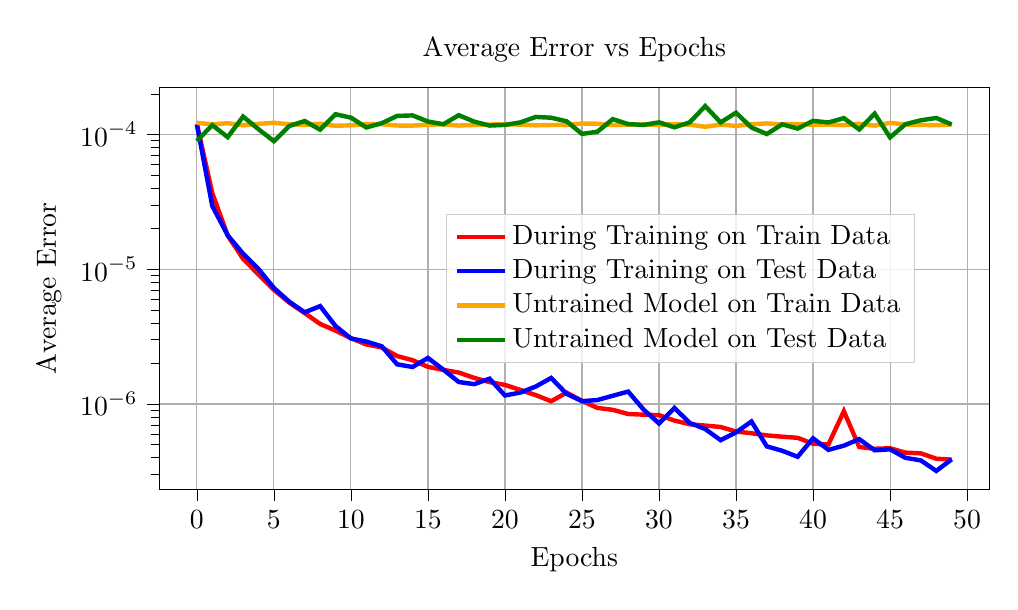
\begin{tikzpicture}

  \definecolor{darkgray176}{RGB}{176,176,176}
  \definecolor{green}{RGB}{0,128,0}
  \definecolor{lightgray204}{RGB}{204,204,204}
  \definecolor{orange}{RGB}{255,165,0}
  
  \begin{axis}[
    width = 1.0\textwidth,
    height = 19em,
  legend cell align={left},
  legend style={
    fill opacity=0.8,
    draw opacity=1,
    text opacity=1,
    at={(0.91,0.5)},
    anchor=east,
    draw=lightgray204
  },
  % log basis y={10},
  tick align=outside,
  tick pos=left,
  title={Average Error vs Epochs},
  x grid style={darkgray176},
  xlabel={Epochs},
  xmajorgrids,
  xmin=-2.45, xmax=51.45,
  xtick style={color=black},
  y grid style={darkgray176},
  ylabel={Average Error},
  ymajorgrids,
  ymin=2.33510655990556e-07, ymax=0.000221454230592227,
  ymode=log,
  ytick style={color=black},
  ytick={1e-08,1e-07,1e-06,1e-05,0.0001,0.001,0.01},
  yticklabels={
    \(\displaystyle {10^{-8}}\),
    \(\displaystyle {10^{-7}}\),
    \(\displaystyle {10^{-6}}\),
    \(\displaystyle {10^{-5}}\),
    \(\displaystyle {10^{-4}}\),
    \(\displaystyle {10^{-3}}\),
    \(\displaystyle {10^{-2}}\)
  }
  ]
  \addplot [ultra thick, red]
table {%
0 0.000119110678497236
1 3.66446620319039e-05
2 1.77629917743616e-05
3 1.19415099106845e-05
4 9.14171869226266e-06
5 7.0352730290324e-06
6 5.64817901249626e-06
7 4.72462261313922e-06
8 3.92743004340446e-06
9 3.50450204678054e-06
10 3.07970799440227e-06
11 2.76725950243417e-06
12 2.6275106392859e-06
13 2.26941324399377e-06
14 2.1133414520591e-06
15 1.88730939498782e-06
16 1.79045071035944e-06
17 1.71247768321336e-06
18 1.56285193497752e-06
19 1.45354010783194e-06
20 1.38544032779464e-06
21 1.27156704365916e-06
22 1.16367743885348e-06
23 1.04827813629527e-06
24 1.21447124001861e-06
25 1.05589560916997e-06
26 9.35082709929702e-07
27 9.04937735413114e-07
28 8.4294913449412e-07
29 8.33415299439366e-07
30 8.2679014212772e-07
31 7.54069617414643e-07
32 7.0767163151686e-07
33 6.91661682594713e-07
34 6.75471369504521e-07
35 6.25178131485882e-07
36 6.06936112035328e-07
37 5.85125235375017e-07
38 5.72119461139664e-07
39 5.61235140139615e-07
40 5.07119239046006e-07
41 5.00920407375816e-07
42 8.84193866568239e-07
43 4.79913239814778e-07
44 4.65450710862569e-07
45 4.69535621050454e-07
46 4.35870873616295e-07
47 4.30478280577518e-07
48 3.92834294871136e-07
49 3.87007872859613e-07
};
\addlegendentry{During Training on Train Data}
\addplot [ultra thick, blue]
table {%
0 0.00011835517216241
1 2.94239616778214e-05
2 1.78588288690662e-05
3 1.30369371618144e-05
4 1.00456127256621e-05
5 7.25863583284081e-06
6 5.73770012124442e-06
7 4.78903893963434e-06
8 5.3246581046551e-06
9 3.79064999833645e-06
10 3.06249035020301e-06
11 2.90575530925707e-06
12 2.68139638137654e-06
13 1.96956534637138e-06
14 1.88275339496613e-06
15 2.19661774281121e-06
16 1.79826713520015e-06
17 1.4568524875358e-06
18 1.40323015784816e-06
19 1.54136819219275e-06
20 1.15701266167889e-06
21 1.21596463031892e-06
22 1.34871140744508e-06
23 1.56057183176017e-06
24 1.1893879445779e-06
25 1.04965113223443e-06
26 1.07065557131136e-06
27 1.15161412850284e-06
28 1.23654535855167e-06
29 9.09538812265964e-07
30 7.17409648132161e-07
31 9.34473348479514e-07
32 7.23355014997651e-07
33 6.52248786536802e-07
34 5.39273003141716e-07
35 6.15782823842892e-07
36 7.42191218705557e-07
37 4.84830366076494e-07
38 4.49736944574397e-07
39 4.06152423693129e-07
40 5.56371048787696e-07
41 4.5693556671722e-07
42 4.90936429287103e-07
43 5.4913465419304e-07
44 4.53623528073877e-07
45 4.61155707398575e-07
46 3.98803734924513e-07
47 3.81665216764304e-07
48 3.18877482641255e-07
49 3.88750692081885e-07
};
\addlegendentry{During Training on Test Data}
\addplot [ultra thick, orange]
table {%
0 0.000121821271022782
1 0.000118786163511686
2 0.000121117249364033
3 0.000116916286060587
4 0.000119748343422543
5 0.000122004646982532
6 0.000118965377623681
7 0.000117821851745248
8 0.000119930613436736
9 0.000115926952275913
10 0.000116842471470591
11 0.000119264717795886
12 0.000119227319373749
13 0.000116418617835734
14 0.000116268653073348
15 0.000118152944196481
16 0.00011861881648656
17 0.000116357769002207
18 0.00011766472744057
19 0.000118461459351238
20 0.000118882810056675
21 0.000118203533929773
22 0.000116807641461492
23 0.000117445903015323
24 0.000117745250463486
25 0.000120490200060885
26 0.000120022261398844
27 0.000117423332994804
28 0.000118374497105833
29 0.000118564435979351
30 0.000118055919301696
31 0.000119002019346226
32 0.00011823955719592
33 0.000113942514872178
34 0.000118257907161023
35 0.00011569067282835
36 0.0001189872782561
37 0.000120693657663651
38 0.000118456307973247
39 0.000119453776278533
40 0.000117906849482097
41 0.000118281546747312
42 0.000117204755952116
43 0.000119701318908483
44 0.000116234936285764
45 0.000121639255667105
46 0.000118501353426836
47 0.000117697200039402
48 0.000117044612125028
49 0.000118546777230222
};
\addlegendentry{Untrained Model on Train Data}
\addplot [ultra thick, green]
table {%
0 8.94988697837107e-05
1 0.000117215560749173
2 9.54625502345152e-05
3 0.000135665308334865
4 0.000109265492937993
5 8.90656738192774e-05
6 0.00011553819058463
7 0.000125691731227562
8 0.000108503714727703
9 0.000141213327879086
10 0.000133093009935692
11 0.000112687819637358
12 0.000121152006613556
13 0.000137145310873166
14 0.000138392802909948
15 0.000124624843010679
16 0.000119010474008974
17 0.000138825504109263
18 0.000124459256767295
19 0.000116323259135243
20 0.000117673094791826
21 0.000122827914310619
22 0.000134805915877223
23 0.000133034307509661
24 0.000125141465105116
25 0.000100915800430812
26 0.000104666156403255
27 0.000129874431877397
28 0.000119255695608445
29 0.000117647301522084
30 0.000122925484902225
31 0.0001129619195126
32 0.000122985773487017
33 0.000162168624228798
34 0.000122765937703662
35 0.000144833509693854
36 0.000112565423478372
37 0.000100688113889191
38 0.000118868752906565
39 0.000110469525679946
40 0.00012610036355909
41 0.000122617464512587
42 0.000132143803057261
43 0.000108827247458976
44 0.000142696153488941
45 9.50354224187322e-05
46 0.000119124881166499
47 0.000127313265693374
48 0.000132477522129193
49 0.000118570867925882
};
\addlegendentry{Untrained Model on Test Data}
\end{axis}

\end{tikzpicture}}\\
  \subfloat[Sixth Scenario: Different Scalars Plus a Single Semi-Positive Definite Matrix$(\tau_k\boldsymbol{S})$]{% This file was created with tikzplotlib v0.10.1.
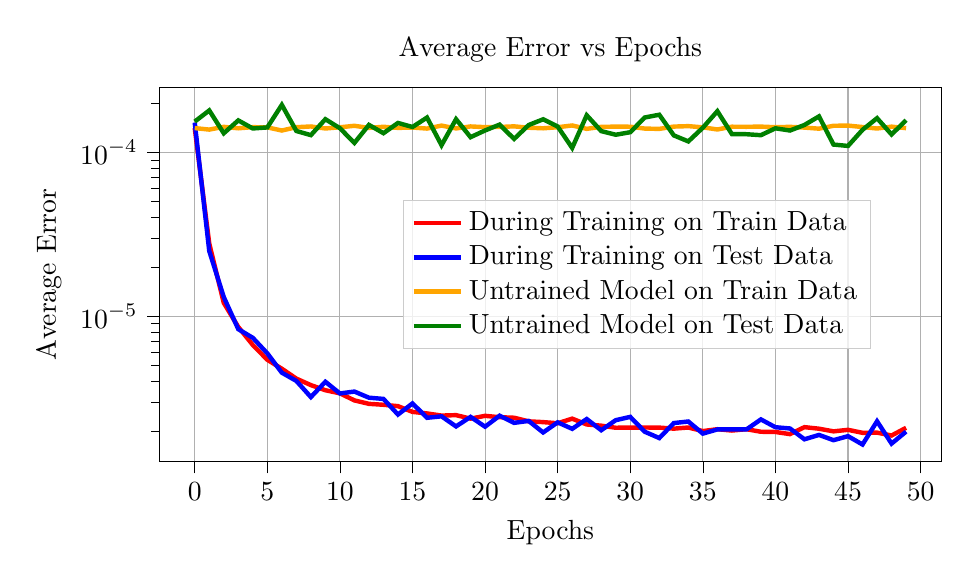
\begin{tikzpicture}

  \definecolor{darkgray176}{RGB}{176,176,176}
  \definecolor{green}{RGB}{0,128,0}
  \definecolor{lightgray204}{RGB}{204,204,204}
  \definecolor{orange}{RGB}{255,165,0}
  
  \begin{axis}[
    width = 0.95\textwidth,
    height = 18em,
  legend cell align={left},
  legend style={
    fill opacity=0.8,
    draw opacity=1,
    text opacity=1,
    at={(0.91,0.5)},
    anchor=east,
    draw=lightgray204
  },
  % log basis y={10},
  tick align=outside,
  tick pos=left,
  title={Average Error vs Epochs},
  x grid style={darkgray176},
  xlabel={Epochs},
  xmajorgrids,
  xmin=-2.45, xmax=51.45,
  xtick style={color=black},
  y grid style={darkgray176},
  ylabel={Average Error},
  ymajorgrids,
  ymin=1.30004957183654e-06, ymax=0.000247303366693065,
  ymode=log,
  ytick style={color=black},
  ytick={1e-07,1e-06,1e-05,0.0001,0.001,0.01},
  yticklabels={
  \(\displaystyle {10^{-7}}\),
  \(\displaystyle {10^{-6}}\),
  \(\displaystyle {10^{-5}}\),
  \(\displaystyle {10^{-4}}\),
  \(\displaystyle {10^{-3}}\),
  \(\displaystyle {10^{-2}}\)
}
  ]
  \addplot [ultra thick, red]
table {%
0 0.000140808770083822
1 2.77877024927875e-05
2 1.20650438475423e-05
3 8.60371164890239e-06
4 6.67991025693482e-06
5 5.42634415978682e-06
6 4.78406172987889e-06
7 4.16472585129668e-06
8 3.80176584258152e-06
9 3.53676637132594e-06
10 3.38710992764391e-06
11 3.06654351334146e-06
12 2.92217282549245e-06
13 2.88355204247637e-06
14 2.82838118437212e-06
15 2.60954288933135e-06
16 2.55327290688001e-06
17 2.47778302764345e-06
18 2.49293429988029e-06
19 2.37284029935836e-06
20 2.46894796873676e-06
21 2.42158648688928e-06
22 2.4035755359364e-06
23 2.28525459533557e-06
24 2.26031443162356e-06
25 2.22407220462628e-06
26 2.37349354392791e-06
27 2.18677610064333e-06
28 2.15019440474862e-06
29 2.08874439522333e-06
30 2.09293762054585e-06
31 2.09529321182345e-06
32 2.09285894925415e-06
33 2.06235563382506e-06
34 2.09541235562938e-06
35 1.99298551706306e-06
36 2.04654361368739e-06
37 2.00757085622172e-06
38 2.0461657186388e-06
39 1.97414806279994e-06
40 1.96775522454118e-06
41 1.90975492841972e-06
42 2.10623920793296e-06
43 2.06045660888776e-06
44 1.98512111637683e-06
45 2.02815704142267e-06
46 1.94528092833934e-06
47 1.95024335880589e-06
48 1.87281955277285e-06
49 2.08697565540206e-06
};
\addlegendentry{During Training on Train Data}
\addplot [ultra thick, blue]
table {%
0 0.000151866624946706
1 2.49946006078972e-05
2 1.30948674268438e-05
3 8.34122874948662e-06
4 7.38843755243579e-06
5 5.93867616771604e-06
6 4.52684344054433e-06
7 4.03162584916572e-06
8 3.21297193295322e-06
9 3.98407746615703e-06
10 3.38162840307632e-06
11 3.47228137798083e-06
12 3.18590946335462e-06
13 3.13101372739766e-06
14 2.51418100560841e-06
15 2.93958305519482e-06
16 2.4015394046728e-06
17 2.45178125624079e-06
18 2.12747499972465e-06
19 2.4323815068783e-06
20 2.11953897633066e-06
21 2.47359025706828e-06
22 2.23747611016734e-06
23 2.29793567996239e-06
24 1.95504912881006e-06
25 2.2525521217176e-06
26 2.05718492907181e-06
27 2.36007554121898e-06
28 2.01702164304152e-06
29 2.32281195167161e-06
30 2.43284330281313e-06
31 1.97447093341907e-06
32 1.80655024450971e-06
33 2.23063898374676e-06
34 2.27990972234693e-06
35 1.92346169569646e-06
36 2.03991839953233e-06
37 2.03988429348101e-06
38 2.03888680516684e-06
39 2.34781578001275e-06
40 2.10382722798386e-06
41 2.0672875962191e-06
42 1.77587082816899e-06
43 1.88824776614638e-06
44 1.75387231138302e-06
45 1.85520821105456e-06
46 1.65030076004768e-06
47 2.28701583182556e-06
48 1.67188488831016e-06
49 1.97793519873812e-06
};
\addlegendentry{During Training on Test Data}
\addplot [ultra thick, orange]
table {%
0 0.00014060313696973
1 0.000137656141305342
2 0.000143065073643811
3 0.000140192554681562
4 0.000142427845275961
5 0.000142034099553712
6 0.000135852737003006
7 0.00014235639537219
8 0.000143847602885216
9 0.00013983370445203
10 0.000142199758556671
11 0.000145203914144076
12 0.00014099404506851
13 0.000143194061820395
14 0.000140986638143659
15 0.000141734140925109
16 0.000139620620757341
17 0.000145604368299246
18 0.000139923329697922
19 0.000143899538670667
20 0.000142461081850342
21 0.000142865843372419
22 0.000144075427670032
23 0.000141339376568794
24 0.000140182426548563
25 0.000142293807584792
26 0.000145876678288914
27 0.000139112686156295
28 0.000143021941767074
29 0.000143526252941228
30 0.000143316239700653
31 0.000139636162202805
32 0.000139017691253684
33 0.000143602766911499
34 0.000144505393109284
35 0.000142094271723181
36 0.000137869006721303
37 0.000143355937325396
38 0.000143186174682342
39 0.000143536293762736
40 0.000142327175126411
41 0.000143050288897939
42 0.00014157967234496
43 0.000139441690407693
44 0.000145230937050655
45 0.000145648096804507
46 0.000142689401400276
47 0.000139756724820472
48 0.000143463927088305
49 0.00014049097080715
};
\addlegendentry{Untrained Model on Train Data}
\addplot [ultra thick, green]
table {%
0 0.000154029330587946
1 0.000180180853931233
2 0.000130726533825509
3 0.000156632129801437
4 0.000139883763040416
5 0.000141912765684538
6 0.000194816995644942
7 0.000135004651383497
8 0.000127355684526265
9 0.000159308925503865
10 0.000140322328661568
11 0.000114190057502128
12 0.000147035854752176
13 0.00013088078412693
14 0.000151125670527108
15 0.000142780350870453
16 0.000163049713592045
17 0.000110557492007501
18 0.00015931720554363
19 0.000123746853205375
20 0.00013601804676
21 0.000147675746120512
22 0.000120715449156705
23 0.000146728663821705
24 0.000159101778990589
25 0.000143717334140092
26 0.00010641503467923
27 0.000168388287420385
28 0.000134773305035196
29 0.000128033978398889
30 0.000132704633870162
31 0.00016315164975822
32 0.000169641323736869
33 0.000126891216496006
34 0.000116580682515632
35 0.000141325872391462
36 0.000178295289515518
37 0.000129308318719268
38 0.00012899779540021
39 0.000127264560433105
40 0.000140162432217039
41 0.000135849215439521
42 0.000146909078466706
43 0.000165729303262196
44 0.00011155797255924
45 0.000109411274024751
46 0.000137256662128493
47 0.00016158472863026
48 0.000128560437588021
49 0.000157007976667956
};
\addlegendentry{Untrained Model on Test Data}
\end{axis}

\end{tikzpicture}}\\
  \caption{Training the \ac{RWF} Algorithm in different Scenarios}
  \label{some easedgxample}
  \end{figure}

%   \clearpage % End the page
}
\afterpage{%
%   \clearpage % Start a new page
\begin{figure}[!htbp]
  \subfloat[Seventh Scenario: Different Matrices$(\boldsymbol{M}_k)$]{% This file was created with tikzplotlib v0.10.1.
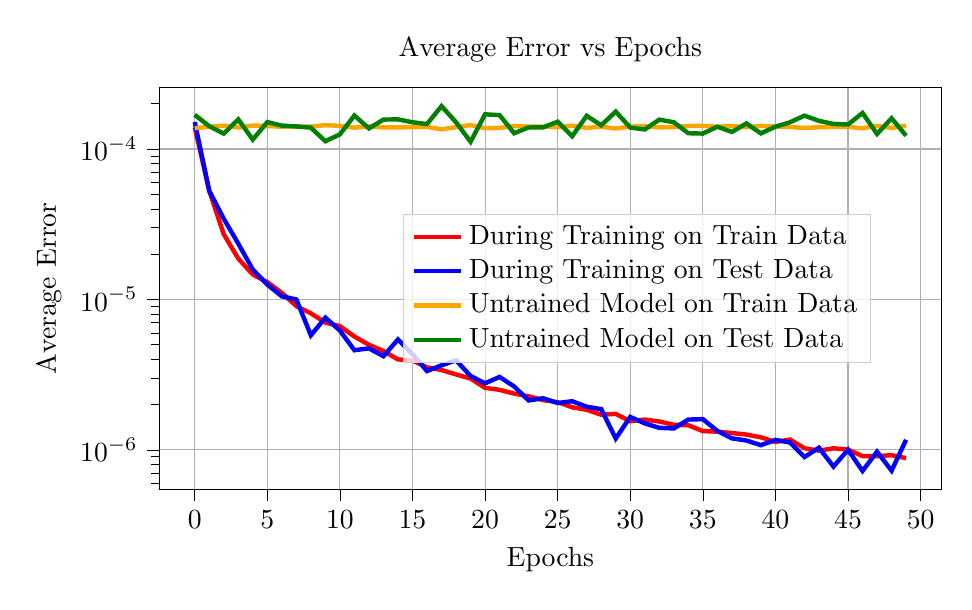
\begin{tikzpicture}

  \definecolor{darkgray176}{RGB}{176,176,176}
  \definecolor{green}{RGB}{0,128,0}
  \definecolor{lightgray204}{RGB}{204,204,204}
  \definecolor{orange}{RGB}{255,165,0}
  
  \begin{axis}[
    width = 0.95\textwidth,
    height = 19em,
  legend cell align={left},
  legend style={
    fill opacity=0.8,
    draw opacity=1,
    text opacity=1,
    at={(0.91,0.5)},
    anchor=east,
    draw=lightgray204
  },
  % log basis y={10},
  tick align=outside,
  tick pos=left,
  title={Average Error vs Epochs},
  x grid style={darkgray176},
  xlabel={Epochs},
  xmajorgrids,
  xmin=-2.45, xmax=51.45,
  xtick style={color=black},
  y grid style={darkgray176},
  ylabel={Average Error},
  ymajorgrids,
  ymin=5.47956319196448e-07, ymax=0.000254691381547786,
  ymode=log,
  ytick style={color=black},
  ytick={1e-08,1e-07,1e-06,1e-05,0.0001,0.001,0.01},
  yticklabels={
    \(\displaystyle {10^{-8}}\),
    \(\displaystyle {10^{-7}}\),
    \(\displaystyle {10^{-6}}\),
    \(\displaystyle {10^{-5}}\),
    \(\displaystyle {10^{-4}}\),
    \(\displaystyle {10^{-3}}\),
    \(\displaystyle {10^{-2}}\)
  }
  ]
  \addplot [ultra thick, red]
table {%
0 0.000139422554639168
1 5.25441355421208e-05
2 2.709246109589e-05
3 1.86883116839454e-05
4 1.4641495909018e-05
5 1.30382604766055e-05
6 1.10479877548642e-05
7 9.03117143025156e-06
8 8.08377171779284e-06
9 7.014934453764e-06
10 6.64117942505982e-06
11 5.66791140954592e-06
12 4.99323004987673e-06
13 4.53997472504852e-06
14 3.99270811612951e-06
15 3.92411902794265e-06
16 3.53491191162902e-06
17 3.39455823450407e-06
18 3.1713191219751e-06
19 2.97965834761271e-06
20 2.58465047409118e-06
21 2.5051617740246e-06
22 2.36605910686194e-06
23 2.27213763537293e-06
24 2.14105693885358e-06
25 2.07581410904822e-06
26 1.91861840903584e-06
27 1.84637030997692e-06
28 1.71315411989781e-06
29 1.73497676314582e-06
30 1.54966937770951e-06
31 1.59103592523024e-06
32 1.54397719143162e-06
33 1.46790443977807e-06
34 1.45789761063497e-06
35 1.33272737912193e-06
36 1.32122954710212e-06
37 1.2942375633429e-06
38 1.26361408092635e-06
39 1.21193875202152e-06
40 1.12860448098218e-06
41 1.17169065561029e-06
42 1.0251166031594e-06
43 9.8811494808615e-07
44 1.02411047464557e-06
45 1.00423574167507e-06
46 9.08802235244366e-07
47 9.08564288693015e-07
48 9.21839614420605e-07
49 8.81109031070082e-07
};
\addlegendentry{During Training on Train Data}
\addplot [ultra thick, blue]
table {%
0 0.000151191532495432
1 5.27330812474247e-05
2 3.43467727361713e-05
3 2.34825092775282e-05
4 1.57967224367894e-05
5 1.25444585137302e-05
6 1.04895107142511e-05
7 9.99405347101856e-06
8 5.77313267058344e-06
9 7.56428335080273e-06
10 6.20858509137179e-06
11 4.59601551483502e-06
12 4.72754800284747e-06
13 4.19237494497793e-06
14 5.41578947377275e-06
15 4.31831585956388e-06
16 3.34092874254566e-06
17 3.64814991371532e-06
18 3.93835989598301e-06
19 3.09812821797095e-06
20 2.76999890047591e-06
21 3.05379262499628e-06
22 2.63992797044921e-06
23 2.13079511013348e-06
24 2.2038937004254e-06
25 2.0483175831032e-06
26 2.10558482649503e-06
27 1.93491723621264e-06
28 1.86590375506057e-06
29 1.18982120511646e-06
30 1.65560504683526e-06
31 1.49886989220249e-06
32 1.40136648951739e-06
33 1.38726443310588e-06
34 1.5903664234429e-06
35 1.600476934982e-06
36 1.33635251131636e-06
37 1.19272579013341e-06
38 1.15448892756831e-06
39 1.07466962617764e-06
40 1.16404714844975e-06
41 1.11877704966901e-06
42 8.96443566489324e-07
43 1.03346019386663e-06
44 7.74358625221794e-07
45 1.00108979950164e-06
46 7.24411620467436e-07
47 9.72342604654841e-07
48 7.2755648261591e-07
49 1.16638921099366e-06
};
\addlegendentry{During Training on Test Data}
\addplot [ultra thick, orange]
table {%
0 0.000137548107886687
1 0.000140638832817785
2 0.000142808101372793
3 0.000138855073601007
4 0.00014315867156256
5 0.000142147371661849
6 0.000140535441460088
7 0.000140832271426916
8 0.000141012889798731
9 0.000143917815876193
10 0.000142426055390388
11 0.000138538351166062
12 0.000141437121783383
13 0.000139053459861316
14 0.000139040130306967
15 0.000139728872454725
16 0.000140273332362995
17 0.00013496758765541
18 0.000139760843012482
19 0.000144059871672653
20 0.000137425566208549
21 0.000137912458740175
22 0.000142265387694351
23 0.000140677715535276
24 0.000141052427352406
25 0.000139516676426865
26 0.00014278301387094
27 0.000138091811095364
28 0.000140507239848375
29 0.000136786737130024
30 0.00014075510262046
31 0.000142040196806192
32 0.000139078518259339
33 0.000139772397233173
34 0.000142270961077884
35 0.000142297969432548
36 0.000140746793476865
37 0.000141959739266895
38 0.000139722877065651
39 0.000142463482916355
40 0.000140872885822318
41 0.00014001976524014
42 0.000137886876473203
43 0.000139517200295813
44 0.00014015486522112
45 0.000140228410600685
46 0.000137308554258198
47 0.00014238734729588
48 0.000138002840685658
49 0.000142704491736367
};
\addlegendentry{Untrained Model on Train Data}
\addplot [ultra thick, green]
table {%
0 0.000168594866408966
1 0.000141678872751072
2 0.000126560087664984
3 0.000157214250066318
4 0.000115438073407859
5 0.000150999199831858
6 0.000142947799758986
7 0.000141304670250975
8 0.000138527931994759
9 0.000112627378257457
10 0.000125072823720984
11 0.000166890022228472
12 0.000136944450787269
13 0.000156815774971619
14 0.000157319751451723
15 0.000150483218021691
16 0.000146467093145475
17 0.00019265255832579
18 0.000150442734593526
19 0.000111669789475854
20 0.000169916238519363
21 0.000167860955116339
22 0.000127240127767436
23 0.000138955030706711
24 0.000139115072670393
25 0.000151672968058847
26 0.000121595592645463
27 0.000166218713275157
28 0.000143689205287956
29 0.000177146794158034
30 0.000138729737955146
31 0.000134799440274946
32 0.00015673965390306
33 0.000150496722199023
34 0.000127258579595946
35 0.000126562154036947
36 0.000140600168379024
37 0.000129729727632366
38 0.000147858329000883
39 0.000126872822875157
40 0.000140709613333456
41 0.000150389416376129
42 0.000166537720360793
43 0.000153616216266528
44 0.000146757418406196
45 0.000145377474837005
46 0.000173495995113626
47 0.000125866179587319
48 0.000159938761498779
49 0.000122543351608329
};
\addlegendentry{Untrained Model on Test Data}
\end{axis}

\end{tikzpicture}}\\  
  \subfloat[Eighth Scenario: Different Semi-Positive Definite Matrices$(\boldsymbol{S}_k)$]{% This file was created with tikzplotlib v0.10.1.
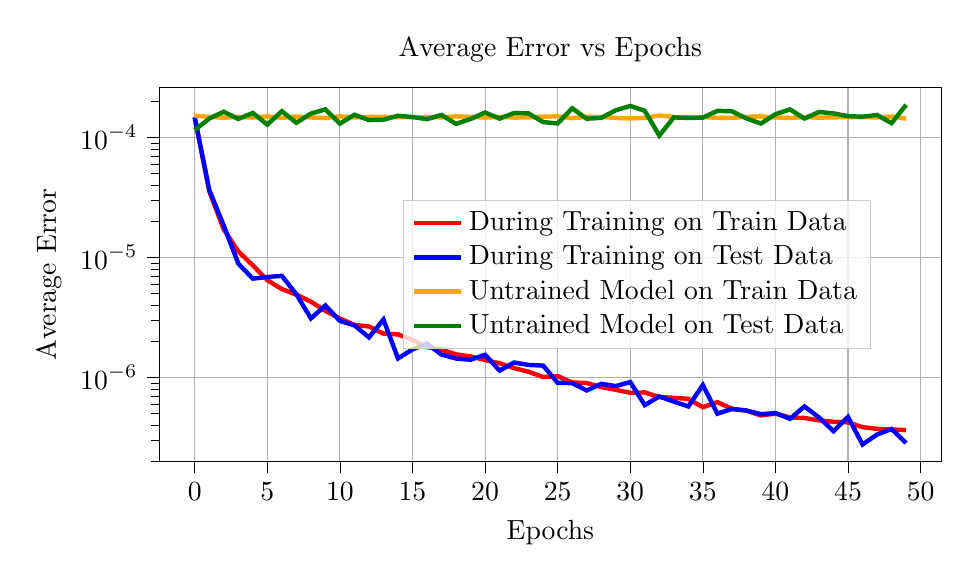
\begin{tikzpicture}

  \definecolor{darkgray176}{RGB}{176,176,176}
  \definecolor{green}{RGB}{0,128,0}
  \definecolor{lightgray204}{RGB}{204,204,204}
  \definecolor{orange}{RGB}{255,165,0}
  
  \begin{axis}[
    width = 0.95\textwidth,
    height = 18em,
  legend cell align={left},
  legend style={
    fill opacity=0.8,
    draw opacity=1,
    text opacity=1,
    at={(0.91,0.5)},
    anchor=east,
    draw=lightgray204
  },
  % log basis y={10},
  tick align=outside,
  tick pos=left,
  title={Average Error vs Epochs},
  x grid style={darkgray176},
  xlabel={Epochs},
  xmajorgrids,
  xmin=-2.45, xmax=51.45,
  xtick style={color=black},
  y grid style={darkgray176},
  ylabel={Average Error},
  ymajorgrids,
  ymin=1.98989848731464e-07, ymax=0.00025862395496495,
  ymode=log,
  ytick style={color=black},
  ytick={1e-08,1e-07,1e-06,1e-05,0.0001,0.001,0.01},
  yticklabels={
    \(\displaystyle {10^{-8}}\),
    \(\displaystyle {10^{-7}}\),
    \(\displaystyle {10^{-6}}\),
    \(\displaystyle {10^{-5}}\),
    \(\displaystyle {10^{-4}}\),
    \(\displaystyle {10^{-3}}\),
    \(\displaystyle {10^{-2}}\)
  }
  ]
  \addplot [ultra thick, red]
  table {%
  0 0.000148013044963591
  1 3.56593227479607e-05
  2 1.7092230336857e-05
  3 1.12235911728931e-05
  4 8.58035764395026e-06
  5 6.45710269964184e-06
  6 5.44462363905041e-06
  7 4.88857358504902e-06
  8 4.2726201172627e-06
  9 3.58169586434087e-06
  10 3.09524739350309e-06
  11 2.73389900939947e-06
  12 2.65521657638601e-06
  13 2.31281637752545e-06
  14 2.27968439503456e-06
  15 2.05286619348044e-06
  16 1.78653704097087e-06
  17 1.69934662608284e-06
  18 1.55517341227096e-06
  19 1.49384698033828e-06
  20 1.3938711163064e-06
  21 1.30992964386678e-06
  22 1.19467654258187e-06
  23 1.11279143766296e-06
  24 1.00586737517006e-06
  25 1.02330841400544e-06
  26 9.0733004753929e-07
  27 8.96316521448171e-07
  28 8.29465079732472e-07
  29 7.87274132107996e-07
  30 7.43528971725027e-07
  31 7.48820809803874e-07
  32 6.85715860981873e-07
  33 6.74960119795287e-07
  34 6.62006982565799e-07
  35 5.64021263471659e-07
  36 6.21000424416707e-07
  37 5.4747005151512e-07
  38 5.2761015467695e-07
  39 4.81172207855707e-07
  40 4.98232964218914e-07
  41 4.6397821051869e-07
  42 4.58541705938842e-07
  43 4.38037005778824e-07
  44 4.26196010039348e-07
  45 4.2150298895649e-07
  46 3.84383071150296e-07
  47 3.72081899513432e-07
  48 3.67385837307665e-07
  49 3.63334208941524e-07
  };
  \addlegendentry{During Training on Train Data}
  \addplot [ultra thick, blue]
  table {%
  0 0.000145961690577678
  1 3.6507273762254e-05
  2 1.83924421435222e-05
  3 8.87434453034075e-06
  4 6.65402694721706e-06
  5 6.85723716742359e-06
  6 7.01677663528244e-06
  7 4.92142953589791e-06
  8 3.10200198327948e-06
  9 3.96965651816572e-06
  10 2.95227073365822e-06
  11 2.71325984613213e-06
  12 2.15284285332018e-06
  13 3.03261163026036e-06
  14 1.43896522786235e-06
  15 1.70873647675762e-06
  16 1.90969149116427e-06
  17 1.54746635416814e-06
  18 1.43470697366865e-06
  19 1.4017372222952e-06
  20 1.54278404806973e-06
  21 1.13814337510121e-06
  22 1.32910520278529e-06
  23 1.26849226944614e-06
  24 1.25276187645795e-06
  25 9.00273789739003e-07
  26 8.95020548341563e-07
  27 7.7743254678353e-07
  28 8.83171367149771e-07
  29 8.45460078835458e-07
  30 9.13137625957461e-07
  31 5.87568308674236e-07
  32 6.92485286890587e-07
  33 6.28680254521896e-07
  34 5.71698194562487e-07
  35 8.63643435877748e-07
  36 4.98133147175395e-07
  37 5.44820807135693e-07
  38 5.29007309069129e-07
  39 4.93094887588086e-07
  40 5.04310378346418e-07
  41 4.50991336720108e-07
  42 5.72123838082916e-07
  43 4.63405569917086e-07
  44 3.56029943304748e-07
  45 4.6835725697747e-07
  46 2.75656987014372e-07
  47 3.33770287852531e-07
  48 3.71070939308993e-07
  49 2.83416682123061e-07
  };
  \addlegendentry{During Training on Test Data}
  \addplot [ultra thick, orange]
  table {%
  0 0.000151286862092093
  1 0.000148271938087419
  2 0.000145962316310033
  3 0.000148140708915889
  4 0.000146270336699672
  5 0.000149768020492047
  6 0.000145538549986668
  7 0.000149274768773466
  8 0.000146568301715888
  9 0.000144949066452682
  10 0.00014968030154705
  11 0.000146915088407695
  12 0.000148198654642329
  13 0.000148643390275538
  14 0.000147157494211569
  15 0.000147706436109729
  16 0.00014777151227463
  17 0.00014694788842462
  18 0.000149669518577866
  19 0.000148425155202858
  20 0.000146184596815147
  21 0.000148376799188554
  22 0.000146324280649424
  23 0.00014655634004157
  24 0.000149089726619422
  25 0.000149657396832481
  26 0.000144709527376108
  27 0.000148061357322149
  28 0.000147991930134594
  29 0.000145307276397943
  30 0.000143848243169487
  31 0.000145373909617774
  32 0.000152415770571679
  33 0.000147752347402275
  34 0.00014776736497879
  35 0.000147837854456156
  36 0.000145569443702698
  37 0.000145633559441194
  38 0.000148161940160207
  39 0.000149608822539449
  40 0.000146714635775425
  41 0.000145101090311073
  42 0.000147954560816288
  43 0.000146047284943052
  44 0.000147063998156227
  45 0.000147197628393769
  46 0.000147608181578107
  47 0.000146761129144579
  48 0.000149398503708653
  49 0.000143366807606071
  };
  \addlegendentry{Untrained Model on Train Data}
  \addplot [ultra thick, green]
  table {%
  0 0.000115061491669621
  1 0.000143547338666394
  2 0.000163512173458003
  3 0.000142517077620141
  4 0.000159814182552509
  5 0.00012783041165676
  6 0.000165362667758018
  7 0.000132426110212691
  8 0.000157876085722819
  9 0.000171300649526529
  10 0.000130172455101274
  11 0.000154473222210072
  12 0.000139474926982075
  13 0.000140412186738104
  14 0.000151597065269016
  15 0.00014767273387406
  16 0.000141933254781179
  17 0.000153813511133194
  18 0.000129606123664416
  19 0.000142261982546188
  20 0.000161294257850386
  21 0.00014334442676045
  22 0.000159681003424339
  23 0.000158348615514114
  24 0.000134108049678616
  25 0.000130705229821615
  26 0.000174892600625753
  27 0.000143100725836121
  28 0.000145519719808362
  29 0.000168184196809307
  30 0.000182958712684922
  31 0.000166574260219932
  32 0.000103557540569454
  33 0.000146681413752958
  34 0.000145311874803156
  35 0.00014605671458412
  36 0.000166460915352218
  37 0.000165033299708739
  38 0.000144075253047049
  39 0.000130360465846024
  40 0.000155840680235997
  41 0.000171156978467479
  42 0.000143605619086884
  43 0.000162815587827936
  44 0.000158585360622965
  45 0.000150236810441129
  46 0.000148762876051478
  47 0.000153807501192205
  48 0.000131454333313741
  49 0.000186694131116383
  };
  \addlegendentry{Untrained Model on Test Data}
  \end{axis}
  
  \end{tikzpicture}
  }\\  
  \caption{Training the \ac{RWF} Algorithm in different Scenarios}
  \label{some examaf}
  \end{figure}

%   \clearpage % End the page
}

